\documentclass[a4paper]{article}
\usepackage[utf8]{inputenc}
\usepackage[T2A]{fontenc}
\usepackage[12pt]{extsizes}

\usepackage[english,russian]{babel} 
\usepackage[left=15mm, top=10mm, right=15mm, bottom=20mm, nohead, nofoot]{geometry} \usepackage{amsmath,amsfonts,amssymb} % математический пакет
\headsep=10mm 


\usepackage{fancybox,fancyhdr} 
\pagestyle{fancy}
\fancyhf{}
\fancyhead[R]{ФТ-104}
\fancyfoot[R]{\thepage} 
\fancyhead[L]{алгем}

\usepackage{xcolor}
\usepackage{hyperref} 
\hypersetup{colorlinks=true, allcolors=[RGB]{010 090 200}} % цвет ссылок 
\newcommand{\lr}[1]{\left({#1}\right)} % команда для скобок
\newtheorem{theorem}{Theorem}

\title{Конспектик к экзамену по алгему}
\author{Васильев Павел}
%\linespread{1}
\usepackage{amsmath}

\usepackage{graphicx}
\usepackage{ifpdf}
\ifpdf
\DeclareGraphicsRule{*}{mps}{*}{}
\fi
\usepackage{graphicx}
\graphicspath{ {images/} }
\begin{document}

{\usefont{T2A}{cmss}{m}{n}
\begin{small}
\section*{Ботаем экзамен по алгему}
\subsection*{Декартово произведение множеств}

\textbf{Прямое, или декартово произведение двух множеств} — множество, элементами которого являются все возможные упорядоченные пары элементов исходных множеств

$\{ (x;y) | x \in A, y \in B \}$

\section*{Понятие отношения на множестве
}
Пусть $M_1, M_2, …, M_n$ – некоторые множества.
Отношением на совокупности этих множеств называется любое подмножество
декартова произведения этих множеств. Если $M_1 = M_2 = … = M_n = M$, то говорят об отношении на множестве M.

\section*{Свойства отношений}

\begin{itemize}
\item \textit{Рефлексивность}: $\forall a \in X (a R a)$
\item \textit{Симметричность}: $\forall a, b \in X (a R b \Rightarrow b R a)$
\item \textit{Антисимметричность}: $\forall a, b \in X (a R b \land b R a \Rightarrow a = b)$
\item \textit{Транзитивность}: $\forall a, b, c \in X (a R b \land b R c => a R c)$


\end{itemize}


\section*{Отношение эквивалентности
}
Отношение на множестве M называется \textbf{отношением
эквивалентности}, если оно \textbf{рефлексивно, симметрично} и \textbf{транзитивно}.

Вот несколько примеров отношений эквивалентности:
\begin{itemize}
\item на любом множестве: отношение равенства;
\item на множестве треугольников: отношение подобия;
\item на множестве действительных чисел: иметь одинаковую целую часть;
\item на множестве вершин графа: быть связанными;
\item на множестве людей: быть одного года рождения.
\end{itemize}


\section*{Теорема о разбиении}
\textbf{Разбиением множества M} называется его представление в виде объединения непустых непересекающихся подмножеств.

\textbf{Теорема о разбиении множества} 
Каждое отношение эквивалентности
задаёт разбиение множества, на котором оно определено. Любое разбиение множества задается некоторым отношением эквивалентности.
\textbf{Доказательство}

Пусть R –
отношение эквивалентности на множестве M. Для каждого элемента a из M построим множество $M_a = \{x | x \in M$ и $x R a\}$. Среди этих множеств могут
оказаться одинаковые. Соберём совокупность всех не совпадающих между
собой множеств $M_a$ и покажем, что их объединение образует разбиение множества M. 

Во-первых, заметим, что каждое множество не пусто, поскольку $a \in M_a$ в
силу рефлексивности отношения R.

Во-вторых, объединение всех выбранных нами множеств совпадает с M,
поскольку каждый элемент из M попадает в подмножество, отмеченное им
самим в роли индекса.

В третьих, покажем, что два различных множества $M_a$ и $M_b$ не пересекаются.
Допустим противное: пусть $c \in M_a \cap M_b$. По построению множеств $M_a$ и $M_b$ это
означает, что $c R a$ и $c R b$. Ввиду симметричности отношения R имеем $a R c$.
Выберем теперь произвольный x из $M_a$. Поскольку $x R a$ и $a R c$, транзитивность
отношения показывает, что $x R c$. Но при этом $c R b$. Применяя ещё раз свойство
транзитивности, получаем $x R b \Rightarrow x \in M_b$. Так как x произвольный, $M_a \subseteq M_b$. В то же время элементы a и b абсолютно
равноправны, поэтому $M_b \subseteq M_a$. Значит, $M_a = M_b$, что противоречит тому, что $M_a$ и $M_b$ различны.

\section*{Отношение порядка}
Отношение на множестве M называется \textbf{отношением
порядка}, если оно \textbf{рефлексивно, транзитивно и антисимметрично}.
Вот несколько примеров отношений порядка:
\begin{itemize}
\item на множестве прямоугольников: содержаться;
\item на множестве действительных чисел: меньше или равно;
\item на множестве сотрудников одного учреждения: быть начальником.
\end{itemize}

\section*{Максимальные и минимальные элементы}
Элемент М множества А, упорядоченного отношением $\unlhd$ называется \textbf{максимальным}, если $\forall a \in A (a \geq M \Rightarrow a = M)$

Элемент m множества А, упорядоченного отношением $\unlhd$ называется \textbf{минимальным}, если $\forall a \in A (a \leq m \Rightarrow a = m)$

\section*{Наибольшие и наименьшие элементы
}
Элемент $a \in A$ называется \textbf{наименьшим}, если $\forall x \in A (a \unlhd x)$\newline
Элемент $a \in A$ называется \textbf{наибольшим}, если $\forall x \in A (a \unrhd x)$

\subsection*{Чем отличается минимальный элемент от наименьшего?}
????????????????????????????????

\section*{Отображения множеств
}

Отображением
множества $M_1$ в множество $M_2$ называют бинарное отношение, определённое на
этих множествах, если первый компонент пары $(a, b) \in M_1 \times M_2$ рассматривается как \textit{аргумент}, а второй – как \textit{значение} для этого аргумента.

\section*{Свойства отображений}

Отображение $f$ множества $M_1$ в множество $M_2$ называется
\textbf{всюду определённым}, если $D(f) = M_1$.

Отображение $f$ множества $M_1$ в множество $M_2$ называется
\textbf{сюръективным}, если $E(f) = M_2$. 

Отображение $f$ множества $M_1$ в множество $M_2$ называется
\textbf{однозначным}, если каждый элемент a из $D(f)$ имеет ровно одно значения в множестве $M_2$:
\begin{equation}
\forall a \in M_1 \forall b \in M_2 \forall c \in M_2 (b  = f(a) \land c = f(a) \Rightarrow b = c)
\end{equation}


Отображение $f$ множества $M_1$ в множество $M_2$ называется
\textbf{инъективным}, если каждый элемент b из $E(f)$ является значением только одного элемента из $M_1$:
\begin{equation}
\forall b \in M_2 \forall a \in M_1 \forall c \in M_1 (b = f(a) \land b = f(x) \Rightarrow a = c)
\end{equation}

Отображение $f$ множества $M_1$ в множество $M_2$ называется
\textbf{биективным}, если оно \textbf{инъективно и сюръективно}. 
%\begin{equation}
%\forall x_1 \in M_1 \forall x_2 \in M_2 \quad x_1 \neq x_2 \Rightarrow f(x_1) \neq f(x_2) \land \forall y \in M_2 \exists x \in M_1 \quad f(x) = y
%\end{equation}

Отображение $f$ множества $M_1$ в множество $M_2$ называется
\textbf{взаимнооднозначным}, если оно \textbf{инъективно, однозначно сюръективно}.

\section*{Обратное отображение
}
Пусть $f$ : $X \rightarrow Y$ - биективное отображение. Тогда каждому $y \in F$ соответствует единичный $x$, который обозначается как $f^{-1} (y)$ b такой, что $f(x) = y$. Таким образом определено отображение $f^{-1}$:$F \rightarrow E$, которое называется \textbf{обратным} отображению $f$.

\section*{Композиция отображений и ее свойства}
\textbf{Композицией отображений} $f$: $X \rightarrow Y$ и $g$:$Y \rightarrow Z$ называется отображение $f \circ g$: $X \rightarrow Z$, обозначающее $f(g(x))$.

Свойства:
\begin{itemize}
\item Композиция двух отображений определена, тогда и только тогда, когда область значений первого отображения совпадает с областью отображения второго.
\item Отображение тогда и только тогда
имеет обратное, когда оно взаимно однозначно (биективно).
\item Из биективности отображения вытекает биективность обратного отображения
\end{itemize}


\subsubsection*{Свойства композиции отображений}

\begin{itemize}
\item \textit{Ассоциативность}: $f \circ (g \circ h) = (f \circ g) \circ h$
\item \textit{Некоммутативность}: $fg \neq gf$

\end{itemize}
\section*{Операции на множестве}
\textbf{Операцией} на множестве M называется всюду
определённая функция из $M^n$ в $M$. Число $n$ называют \textit{арностью}, или
\textit{местностью}, данной операции.
Вот несколько примеров операций:
\begin{itemize}
\item на множестве натуральных чисел: сложение двух чисел; это бинарная
(двуместная) операция;
\item на множестве целых чисел: нахождение числа, противоположного
данному; это унарная (одноместная) операция;
\item на множестве рациональных чисел: нахождение среднего арифметического
n чисел; это n-арная (n-местная) операция;
\item на множестве подмножеств данного множества: операция пресечения
подмножеств; это бинарная операция.
\end{itemize}

\section*{Свойства операций}
\begin{itemize}
\item \textit{Коммутативность} операции $\circ$: $\forall x, y \in M \quad (x \circ y = y \circ x)$
\item \textit{Ассоциативность} операции $\circ$: $\forall x, y, z \in M \quad (x \circ y) \circ z = x \circ (y \circ z)$
\item Элемент $e$ из M называется \textit{нейтральным} относительн операции $\circ$: $\forall x \in M \quad x \circ e = e \circ x = x$
\item Элемент $y$ из M называется \textit{симметричным} относительн операции $\circ$: $x \circ y = y \circ x = e$
\end{itemize}

\section*{Понятие полугруппы, группы}
\textbf{Полугруппа} - множество, на котором определена ассоциативная операция.

Примеры полугрупп:
\begin{itemize}
\item множество натуральных чисел как относительно операции сложения, так и
операции умножения;
\item множество отрицательных целых чисел относительно сложения;
\item булеан множества M относительно операций объединения и пересечения;
\item множество всюду определённых функций, отображающих множество M в
себя, относительно операции композиции
\end{itemize}

\textbf{Группа} - множество, на котором определена ассоциативная операция, имеется нейтральный элемент и каждый элемент обладает симметричным (множество, на котором определена ассоциативная операция)

Примеры групп:
\begin{itemize}
\item множество целых чисел относительно операции сложения;
\item множество положительных рациональных чисел относительно операции
умножения;
\item множество ненулевых действительных чисел относительно операции
умножения;
\item множество взаимно-однозначных отображений произвольного множества M на себя.
\end{itemize}

\section*{Симметрическая группа}
\textbf{Симметрической группой ($S_n$)} называется множество \textit{подстановок} на множестве (подстановка на множестве $M_n$ - взаимнооднозначное отображение множества $M_n$ на себя)

\section*{Разрешимость уравнений в группе
}
???????????????????????????????????
\section*{Кольца и их свойства}
\textbf{Кольцо} - множество M, на котором определены две бинарные операции $\circ$ и $*$, удовлетворяющие следующим условиям:
\begin{itemize}
\item M - группа относительно $\circ$
\item $*$ дистрибутивна относительно $\circ$
\end{itemize}

Примеры:
\begin{itemize}
\item множество целых чисел относительно операций сложения и умножения;
\item множество действительных чисел относительно операций сложения и
умножения;
\item множество многочленов с действительными коэффициентами
относительно операций сложения и умножения;
\item множество функций из R в R относительно операций сложения и умножения.
\end{itemize}

\section*{Области целостности и поля}
\textbf{Область целостности} - коммутативное ассоциатовное кольцо без \textit{делителей нуля} (Ненулевые элементы $a$ и $b$ кольца K называются \textit{делителями нуля}, если $ab = 0$).

\textbf{Поле} - коммутативное ассоциативное кольцо с 1, каждый ненулевой элемент которого обратим.


%===========================================================
%===========================================================
%===========================================================
%===========================================================
%===========================================================


\section*{Понятие вектора}
\textbf{Вектор} — это элемент векторного пространства (некоторого множества с двумя операциями на нём, которые подчиняются восьми аксиомам).

\textbf{Вектором} называется отрезок,
концы которого упорядочены. Первый из его концов
называется началом, второй – концом вектора.

\section*{Операции сложения и умножения векторов и их свойства}

Свойства:
\begin{itemize}
\item \textit{Коммутативность}: $\vec{a} + \vec{b} = \vec{b} + \vec{a}$
\item \textit{Ассоциативность сложения} $(\vec{a} + \vec{b}) + \vec{c} = \vec{a} + (\vec{b}+\vec{c})$
\item \textit{Нейтральный элемент} относительно сложения $\vec{0}$: $\vec{a} + \vec{0} = \vec{a}$
\item \textit{Противоположный вектор} для любого ненулевого относительно умножения: $\vec{a}+(-\vec{a}) = \vec{0}$
\item \textit{Ассоциативность умножения}: $(\lambda \cdot \eta) \cdot \vec{a} = \lambda \cdot ( \eta \cdot \vec{a})$
\item \textit{Дистрибутивность} умножения относительно сложения: $\lambda \cdot (\vec{a} + \vec{b}) = \lambda \cdot \vec{a} + \lambda \cdot \vec{b}$, $(\lambda + \eta) \cdot \vec{a} = \lambda \cdot \vec{a} + \eta \cdot \vec{a}$
\item \textit{Нейтральный элемент} относительно умножения: $1 \cdot \vec{a} = \vec{a}$
\end{itemize}
\section*{Коллинеарность векторов}
Два вектора $\vec{a}$ и $\vec{b}$ \textbf{коллинеарны}, если $\exists t$: $\vec{a} = t \cdot \vec{b}$.

Два вектора \textbf{коллинеарны}, если отношения их координат равны.

Два вектора \textbf{коллинеарны}, если их векторное произведение равно нулевому вектору.

\section*{Базис на плоскости}
\textbf{Базисом} на плоскости называется любая упорядоченная пара линейно независимых векторов, принадлежащих этой плоскости. 

\subsubsection*{Теорема о разложении вектора по базису на плоскости}

Пусть $(\vec{a},\vec{b})$ – базис некоторой плоскости, а $\vec{x}$ – вектор, лежащий в этой
плоскости. Тогда существуют, и притом единственные, числа $t_1$ и $t_2$ такие,
что
\begin{equation}
\vec{x} = t_1 \vec{a} + t_2 \vec{b}
\end{equation}

\subsubsection*{Доказательство}
Отложим вектора $\vec{a}$, $\vec{b}$ и $\vec{x}$ от некоторой точки O нашей
плоскости и обозначим концы полученных направленных отрезков через A, B и M соответственно.

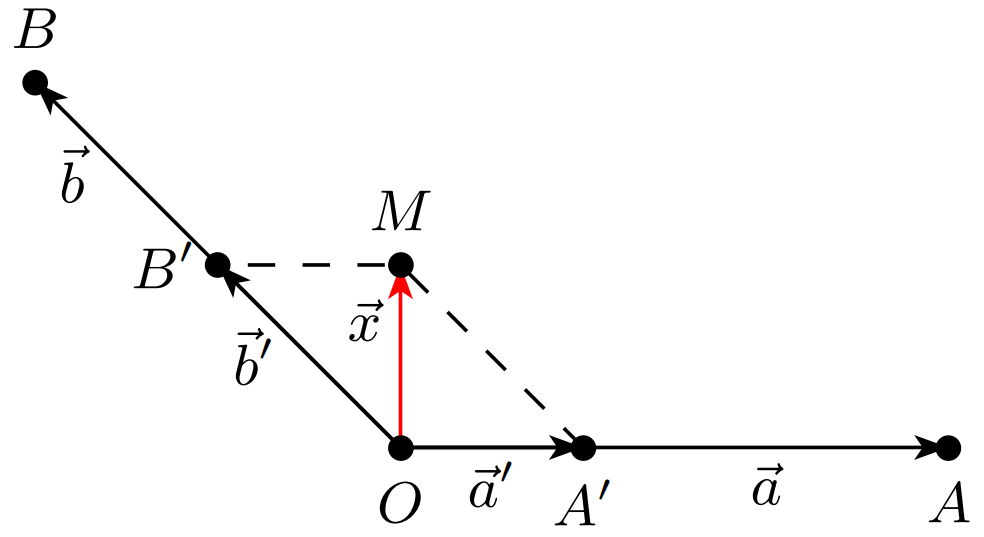
\includegraphics[width=10cm]{t1}

Спроектируем точку M на прямую OA параллельно прямой OB и на прямую OB параллельно прямой OA. Обозначим полученные точки через $A'$ и $B'$ соответственно и положим  $\vec{a}' := \overrightarrow{OA}'$ и $\vec{b}' := \overrightarrow{OB}'$. Ясно, что $\vec{a}' \parallel \vec{a}$ и $\vec{b}' \parallel \vec{b}$. Поскольку $\vec{a}$, $\vec{b} \neq \vec{0}$, по критерию коллинеарности векторов $\vec{a}' = t_1 \vec{a}$ и $\vec{b}' = t_1 \vec{b}$ для некоторых чисел $t_1$ и $t_2$.
Тогда $\vec{x} = t_1 \vec{a} + t_2 \vec{b}$.

Осталось доказать единственность. Пусть $\vec{x} = s_1 \vec{a} + s_2 \vec{b}$ для некоторых  чисел $s_1$ и $s_2$. Вычитая это равенство из равенства $\vec{x} = t_1 \vec{a} + t_2 \vec{b}$ имеем $(t_1 - s_1) \vec{a} + (t_2 - s_2) \vec{b} = \vec{0}$. Если $t_1-s_1 \neq 0$, то $\displaystyle \vec{A} = - \frac{t_2 - s_2}{t_1 - s_1} \cdot \vec{b} \parallel \vec{b}$, противоречие. Следовательно, $t_1 - s_1 = 0$, то есть $t_1 = s_1$. 

\section*{Действия с векторами в координатной форме}

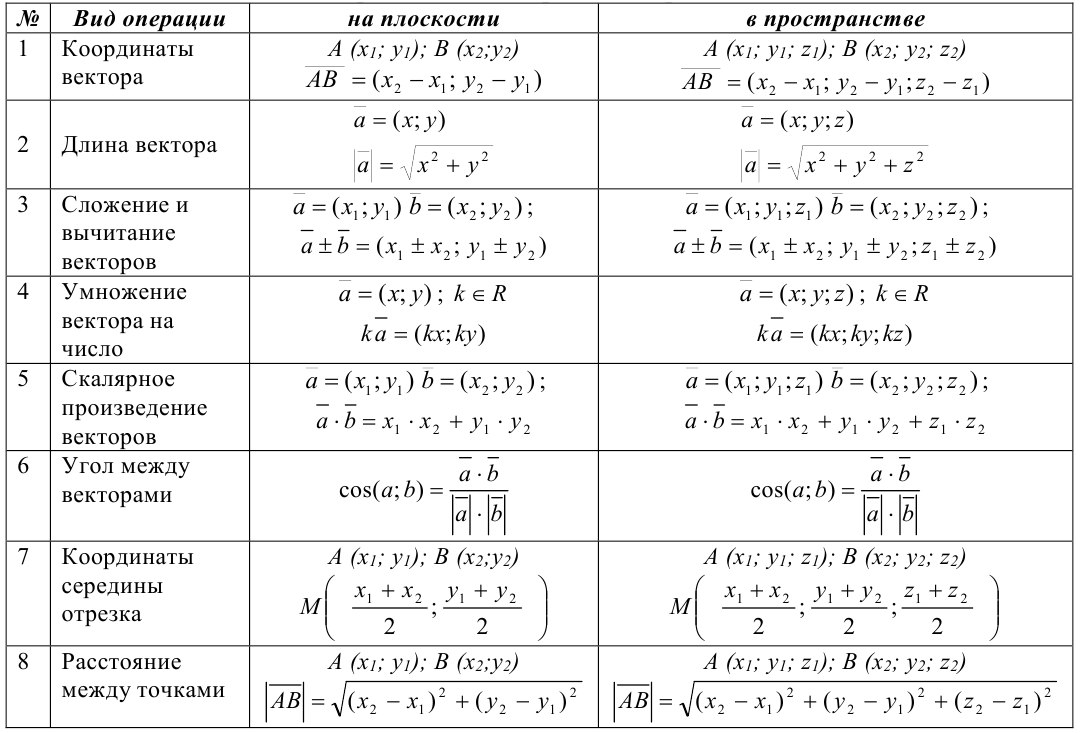
\includegraphics[width=18cm]{t2}
\section*{Компланарность векторов}
\textbf{Компланарные векторы} — это векторы, которые параллельны одной плоскости или лежат на одной плоскости. 

Условия компланарности векторов:
\begin{itemize}
\item Для 3-х векторов выполняется условие: если смешанное произведение 3-х векторов равно нулю, то эти три вектора компланарны
\item Для 3-х векторов выполняется условие: если три вектора линейно зависимы, то они компланарны.
\item если среди векторов не более 2-х линейно независимых векторов, то они компланарны.
\end{itemize}
\section*{Базис пространства}
\textbf{Базисом пространства }называется упорядоченная тройка некомпланарных
векторов

\subsubsection*{Теорема о разложении вектора по базису в пространстве}

Пусть $( \vec{a}, \vec{b}, \vec{c})$ - базис пространства, а $\vec{x}$ - произвольный вектор. Тогда существуют единственные $t_1$, $t_2$, $t_3$ такие, что
\begin{equation}
\vec{x} = t_1 \vec{a} + t_2 \vec{b} + t3 \vec{x}
\end{equation}

\subsubsection*{Доказательство}

Отложим вектора $\vec{a}$, $\vec{b}$  и $\vec{c}$ от некоторой точки О и обозначим концы полученных направленных отрезков через A, B, C и M соответственно.

Поскольку $\vec{a}$ и $\vec{b}$ неколлинеарны, существует единственная плоскость $\pi$, проходящая через точки O, A и B. Спроектируем точку M на плоскость $\pi$ параллельно прямой OC и  на прямую OC параллельно плоскоси $\pi$. 

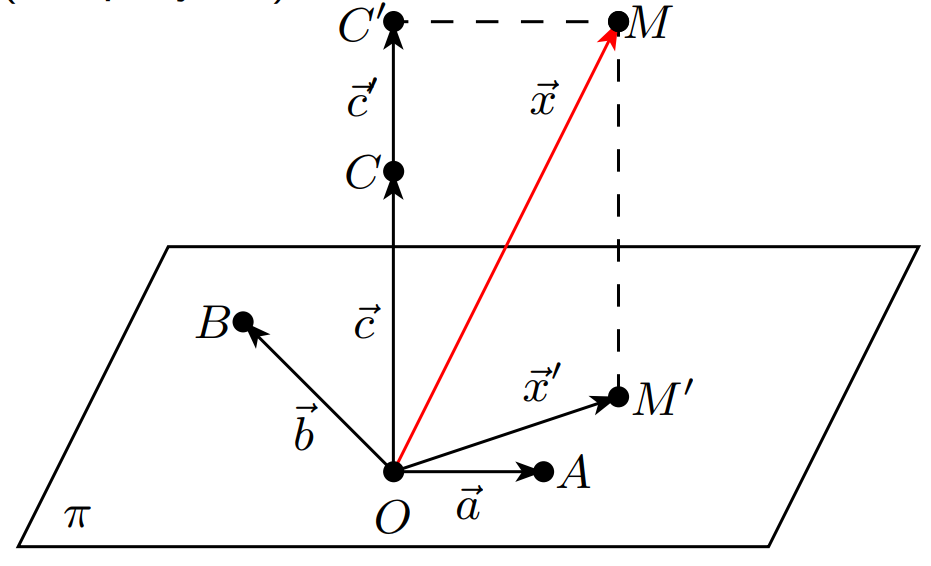
\includegraphics[width=12cm]{t3}

Обозначим полученные точки как $M'$ и $C'$ и положии $\vec{x}' := \overrightarrow{OM}'$ и $\vec{c}' := \overrightarrow{OC}'$. По теореме о разложении вектора по базису на плоскости  $\vec{x} = t_1 \vec{a} + t_2 \vec{b}$ для некоторых $t_1$ и $t_2$. Далее $\vec{c}' \parallel \vec{c} \neq \vec{0}$, откуда $\vec{c}' = t_3 \vec{c}$ для некоторого $t_3$. Тогда $\vec{x} = \vec{x} + \vec{c}' = t_1 \vec{a} + t_2 \vec{b} + t_3 \vec{c}$. Существование чисел $t_1$, $t_2$, $t_3$ с требуемыми свойствами доказано.
Осталось доказать их единственность. Пусть $\vec{x} = s_1 \vec{a} + s_2 \vec{b} + s_3 \vec{c}$ для некоторых $s_1$, $s_2$ и $s_3$. Вычитая это равенство их равенства $\vec{x} = t_1 \vec{a} + t_2 \vec{b} + t_3 \vec{c}$, получим  
\begin{equation}
(t_1 -s_1) \vec{a} + (t_2 - s_2)\vec{b} + (t_3 - s_3) \vec{c} = \vec{0}
\end{equation}
Если $\displaystyle t_1 -s_1 \neq	0$, то $\vec{a} = - \frac{t_2 - s_2}{t_1 - s_1} \cdot \vec{b} - \frac{t_3 - s_3}{t_1 - s_1} \cdot \vec{c}$. Но тогда вектора $\vec{a}$, $\vec{b}$ и $\vec{c}$ компланарны, что противоречит условию $\Rightarrow t_1 - s_1 = 0 \Rightarrow t_1 = s_1$. Аналогично $t_2 = s_2$ и $t_3 = s_3$.


\section*{Скалярное произведение векторов}

\textbf{Скалярным произведением} ненулевых векторов называется число, равное
произведению длин этих векторов на косинус угла между ними. Скалярное
произведение нулевого вектора на любой вектор по определению равно 0.
Скалярное произведение векторов ~a и ~b обозначается через $\vec{a} \vec{b}$
\begin{equation}
\vec{a} \vec{b} = |\vec{a}| \cdot | \vec{b} | \cdot \cos(\widehat{\vec{a}, \vec{b}})
\end{equation}

Свойства:
\begin{itemize}
\item $\vec{a} \vec{b} = \vec{b} \vec{a}$
\item $(\vec{a} + \vec{b}) \vec{c} = \vec{a} \vec{c} + \vec{b} \vec{c}$
\item $(t \vec{a}) \vec{b} = t (\vec{a} \vec{b})$
\item $\vec{a} \vec{a} \geq 0$, причём $\vec{a} \vec{a} = 0$ только тогда, когда $\vec{a} = \vec{0}$.
\end{itemize}

\section*{Компонента вектора на прямую и проекция вектора на ось
}
Если $\vec{a} = x \vec{i} + y \vec{j} + z \vec{z}$, то $x \vec{i}$, $x \vec{i}$ и $x \vec{i}$ - \textbf{компоненты} этого вектора.

\textbf{Проекция} вектора на ось – это вектор, началом и концом которого являются соответственно проекции начала и конца заданного вектора.

\section*{Свойства компоненты, проекции и скалярного произведения}

Свойства проекций (пусть векторы $\vec{a}$ и $\vec{b}$ проецируются на прямую $l$):
\begin{itemize}
\item $pr_l (\vec{a} + \vec{b}) = pr_l \vec{a} + pr_l \vec{b}$
\item $pr_l (t \vec{a}) = t pr_l \vec{a}$
\end{itemize}

\section*{Векторное и смешанное произведения векторов}

\textbf{Упорядоченная тройка} некомпланарных векторов $(\vec{u}, \vec{v}, \vec{w})$  называется
правой, если из конца вектора $\vec{w}$ поворот от $\vec{u}$ к $\vec{v}$ по наименьшему углу
выглядит происходящим против часовой стрелки, и левой – в противном случае. Правую тройку векторов называют также положительно
ориентированной, а левую – отрицательно ориентированной.

\textbf{Векторным произведением} неколлинеарных векторов $\vec{a}$ и $\vec{b}$ называется
вектор $\vec{c}$ такой, что:
\begin{itemize}
\item $| \vec{c}| = | \vec{a} | \cdot | \vec{b} | \cdot \sin (\widehat{\vec{a}, \vec{b}})$
\item $\vec{c}$ ортогонален к векторам $\vec{a}$ и $\vec{b}$
\item тройка $(\vec{a}, \vec{b}, \vec{c})$ - правая.
\end{itemize}

Если $\vec{a}, \vec{b}$ и $\vec{c}$ - произвольные вектора, а $t$ - произвольное число, то
\begin{itemize}
\item $\vec{a} \times \vec{b} = -\vec{b} \times \vec{a}$ (антикоммутативность)
\item $(t \vec{a}) \times \vec{b} = \vec{a} \times (t \vec{b}) = t ( \vec{a} + \vec{b})$
\item $(\vec{a} +\vec{b}) \times \vec{c} = \vec{a} \times \vec{c} + \vec{b} \times \vec{c}$
\item $\vec{a} \times (\vec{b} + \vec{c}) = \vec{a} \times \vec{b} +\vec{a} \times \vec{c}$
\end{itemize}

\textbf{Смешанным произведением} векторов $\vec{a}, \vec{b}$ и $\vec{c}$ называется число, равное
скалярному произведению векторного произведения векторов $\vec{a}$ и $\vec{b}$
на вектор $\vec{c}$ (обозначается $\vec{a} \vec{b} \vec{c}$.
Таким образом, $\vec{a} \vec{b} \vec{c} := (\vec{a} \times \vec{b}) \vec{c}$.

\textbf{Критерий компланарности векторов}. Вектора $\vec{a}, \vec{b}$ и $\vec{c}$ компланарны тогда и только тогда, когда их смешанное
произведение равно нулю.

\textbf{Доказательство.} Необходимость. Предположим, что вектора $\vec{a}, \vec{b}$ и $\vec{c}$ компланарны. Если $\vec{a} \parallel \vec{b}$, то $\vec{a} \times \vec{b} = \vec{0}$, и потому $\vec{a} \vec{b} \vec{c} = (\vec{a} \times \vec{b} ) \vec{c} = \vec{0}$. \\
Пусть теперь $\vec{a} \nparallel \vec{b}$. Отложим вектора $\vec{a}, \vec{b}$ и $\vec{c}$ от одной точки. Тогда они будут лежать в некоторой плоскости. Вектор $\vec{a} \times \vec{b}$ ортогонален этой плоскости а значит и вектору $\vec{c}$. Следовтельно $\vec{a} \vec{b} \vec{c} = (\vec{a} \times \vec{b} ) \vec{c} = \vec{0}$.

Достаточность. Если $\vec{a} \parallel \vec{b}$, то компланарность очевидна Пусть теперь $\vec{a} \nparallel \vec{b}$. Будем считать что вектора $\vec{a}, \vec{b}$ и $\vec{c}$ отложены от отдной и той же точки Пусть $\vec{a} \vec{b} \vec{c} = 0$. Это означает что $(\vec{a} \times \vec{b}) \vec{c} = 0$. Следовательно $\vec{a} \times \vec{b}$ ортогонален вектору $\vec{c}$. Но вектор $\vec{a} \times \vec{b}$ ортогонален плоскости $\delta$, образованной векторами $\vec{a}$ и $\vec{b}$. Поскольку $\vec{c}$ ортогонален этому вектору, то он лежитт в $\delta$. А это означает, что вектора $\vec{a}, \vec{b}$ и $\vec{c}$ компланарны.

\textbf{Теорема  (геометрический смысл смешанного произведения)} Объем параллелепипеда, построенного на трех некомпланарных векторах,
равен модулю их смешанного произведения.

\textbf{Доказательство}. Пусть $\vec{a}, \vec{b}$ и $\vec{c}$ - три некомпланарных вектора. Предположим сначала, что тройка $(\vec{a}, \vec{b}, \vec{c})$ - правая. 

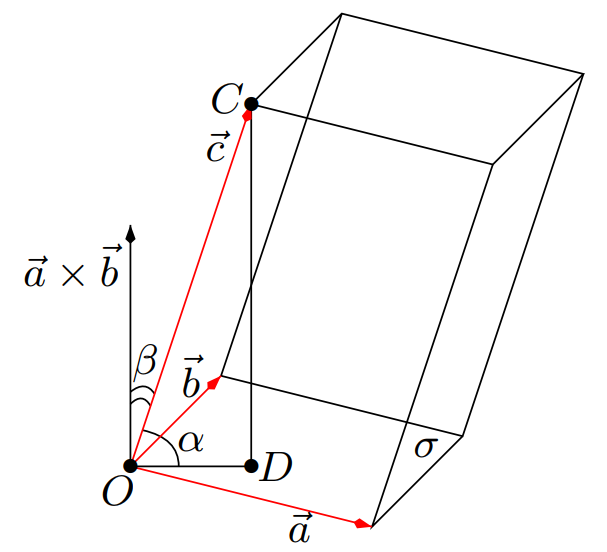
\includegraphics[width=11cm]{t4}


Отложим вектора $\vec{a}, \vec{b}$ и $\vec{c}$ от точки O. Пусть точка С такая, что $\overrightarrow{OC} = \vec{c}$, а D - проекция точки C на плоскость векторов $\vec{a}$ и $\vec{b}$, которую обозначим через $\sigma$. Учитывая, что $\alpha + \beta = \frac{\pi}{2}$ и потому $\sin \alpha = \cos \beta$, и юзая геометрический смысл векторного произведения, имеем 
\begin{equation}
V = S \cdot h =  | \vec{a} \times \vec{b} | \cdot | CD | = |\vec{a} \times \vec{b}| \cdot | \vec{c} | \cdot \sin \alpha = |\vec{a} \times \vec{b}| \cdot | \vec{c} | \cdot \cos \beta = ( \vec{a} \times \vec{b}) \vec{c} = \vec{a} \vec{b} \vec{c}.
\end{equation}

Пусть теперь тройка $\vec{a}, \vec{b}$ и $\vec{c}$ левая. Тогда $\alpha = \beta - \frac{\pi}{2}$, откуда $\sin \alpha = - \cos \beta$.

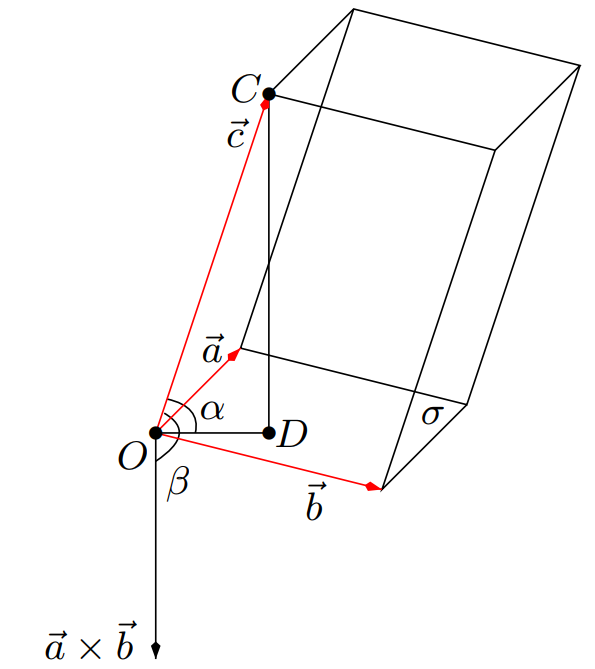
\includegraphics[width=10cm]{t5}

\begin{equation}
V = S \cdot h = | \vec{a} \times \vec{b} | \cdot | CD | = | \vec{a} \times \vec{b} | \cdot | \vec{c} | \cdot \sin \alpha = - | \vec{a} \times \vec{b} | \cdot | \vec{c} | \cdot \cos \beta = - (\vec{a} \times \vec{b}) \vec{c} = -\vec{a} \vec{b} \vec{c}
\end{equation}

\begin{itemize}
\item $\vec{a} \vec{b} \vec{c} = V > 0$, если тройка правая
\item $\vec{a} \vec{b} \vec{c} = -V < 0$, если тройка левая
\end{itemize}


Вот еще свойства (пусть $\vec{a}, \vec{b}, \vec{c}, \vec{d}$ - произвольные вектора, а $t$ - число)
\begin{itemize}
\item $\vec{a} \vec{b} \vec{c} = \vec{b} \vec{c} \vec{a} = \vec{c} \vec{a} \vec{b} = -\vec{a} \vec{c} \vec{b} = -\vec{c} \vec{b} \vec{a} = -\vec{b} \vec{a} \vec{c}$
\item $(t\vec{a}) \vec{b} \vec{c} = \vec{a} (t \vec{b}) \vec{c} = \vec{a} \vec{b} (t \vec{c}) = t (\vec{a} \vec{b} \vec{c})$
\item $(\vec{a} + \vec{b}) \vec{c} \vec{d} = \vec{a} \vec{c} \vec{d} + \vec{b} \vec{c} \vec{d} $
\item $\vec{a} (\vec{b} + \vec{c}) \vec{d} = \vec{a} \vec{b} \vec{d} + \vec{a} \vec{c} \vec{d}$
item $\vec{a} \vec{b} (\vec{c} + \vec{d}) = \vec{a} \vec{b} \vec{c} + \vec{a} \vec{b} \vec{d}$
\end{itemize}


\section*{Системы координат на плоскости и в пространстве}
\textbf{Координатами} точки М называются координаты её радиус-вектора.

Точка А делит отрезок $M_0 M_1$ внутренним образом в отношении $\lambda$, если $\displaystyle \frac{M_0 A}{A M_1} = \lambda$,\newline внешним образом, если $\displaystyle \frac{M_0 A}{A M_1} = -\lambda$

\begin{equation}
\displaystyle A \left( \frac{x_0 + \lambda x_1}{1 + \lambda}; \frac{y_0 + \lambda y_1}{1 + \lambda}; \frac{z_0 + \lambda z_1}{1+\lambda}\right)
\end{equation}



\section*{Виды уравнений прямой на плоскости}

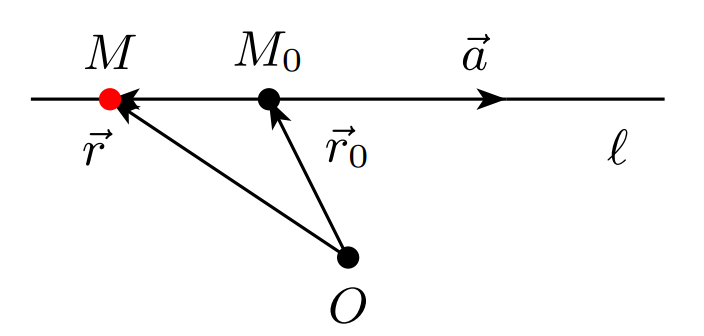
\includegraphics[width=11cm]{t6}

Любая точка на прямой может быть задана как $\vec{r} = \vec{r_0} + t\vec{a}, t \in \mathbb{R}, \vec{r_0} = (x_0, y_0), \vec{r} = (x,y), \vec{a} = (r, s)$ 

Уравнения прямой:
\begin{enumerate}


\item Параметрическое: $
 \begin{cases}
   x = x_0 + tr,
   \\
   y = y_0 + ts
 \end{cases}$

\item Каноническое: $\displaystyle \frac{x-x_0}{r} = \frac{y-y_0}{s}$
\item Общее: $Ax + By + C = 0, A^2 + B^2 \neq 0$
\end{enumerate}

\textbf{Определение.} Пусть прямая $l$ задана уравнением $Ax + By + C = 0$. Тогда вектор $\vec{n} = (A, B)$ называется \textbf{главным вектором} прямой $l$.

\textbf{Замечание.} Главный вектор прямой не коллинеарен этой прямой.

\textbf{Доказательство}. Пусть прямая $l$ задана уравнением $Ax + By + C = 0$, $\vec{n} = (A, B), M_0 (x_0, y_0) \in l$, то есть $Ax_0 + By_0 + C = 0$. Отложим вектор $\vec{n}$ от точки $M_0$. Концом соответствующего направленного отрезка будет точка $M_1(x_0 + A, y_0 + B)$. Подставив координаты этой точки в левую часть уравнения прямой, получим $A (x_0 + A) + B(y_0 + B) + C = Ax_0 + By_0 + C + A^2 + B^2 = A^2 + B^2 \neq 0$.

Таким образом, $M_1 \notin l$. Поскольку $M_0 \in l$, а $\overrightarrow{M_0 M_1} = \vec{n}$, это означает, что вектор $\vec{n}$ и прямая $l$ не коллинеарны.

\section*{Взаимное расположение прямых на плоскости}

\textbf{Теорема}. Пусть прямые $l_1$ и $l_2$ заданы уравнениями \begin{itemize}
\item $A_1x+B_1y+C_1 = 0$
\item $A_2x+B_2y+C_2 = 0$
\end{itemize}. Тогда \begin{enumerate}
\item $l_1$ и $l_2$ пересекаются $\displaystyle \Leftrightarrow \frac{A_1}{A_2} \neq \frac{B_1}{B_2}$
\item $\displaystyle l_1 \parallel l_2$ и $\displaystyle l_1 \neq l_2 \Leftrightarrow \frac{A_1}{A_2} = \frac{B_1}{B_2} \neq \frac{C_1}{C_2}$
\item $\displaystyle l_1 = l_2 \Leftrightarrow \frac{A_1}{A_2} = \frac{B_1}{B_2} = \frac{C_1}{C_2}$
\end{enumerate}

\textbf{Доказательство} (в ПСК).

$\displaystyle \frac{A_1}{A_2} = \frac{B_1}{B_2}$ (условие параллельности нормальных векторов в ПСК). 

Направляющие вектора: $\vec{a_1} = (-B_1, A_1), \vec{a_2} = (-B_2, A_2)$. \newline $l_1 \parallel l_2$ или $\displaystyle l_1 = l_2 \Leftrightarrow a_1 \parallel a_2 \Leftrightarrow \frac{-B_1}{-B_2} = \frac{A_1}{A_2}$, откуда следует утверждение 1.

Пусть $t = \frac{A_1}{A_2} = \frac{B_1}{B_2}$. 

$A_1 = tA_2$

$B_1 = tB_2$

$t \neq 0$, иначе $A_1 = B_1 = 0$

Получаем $
\begin{cases}
   A_1x+B_1y+C_1 = 0
   \\
   A_2x + B_2y+C_2 = 0
 \end{cases}
$

$
\begin{cases}
   tA_2x+tB_2y+C_1 = 0
   \\
   A_2x + B_2y+C_2 = 0
 \end{cases}
$

$
\begin{cases}
   tA_2x+tB_2y+C_1 = 0
   \\
   tA_2x + tB_2y+tC_2 = 0
 \end{cases}
$

$C_1 - tC_2 = 0$

$C_1 = tC_2$, то есть только при $\displaystyle t=\frac{C_1}{C_2}$ система имеет решение, откуда следуют утверждения 2 и 3.

\section*{Нормальное уравнение прямой на плоскости}
??????????????????????????????????????????????

\section*{Отклонение точки от прямой}
\textbf{Теорема (о полуплоскостях)}. Пусть $M(x', y')$ - точка плоскости. Если $M \in \lambda$, то $Ax' + By' + C > 0$, а если $M \in \mu $, то $Ax' + By' + C < 0$ 

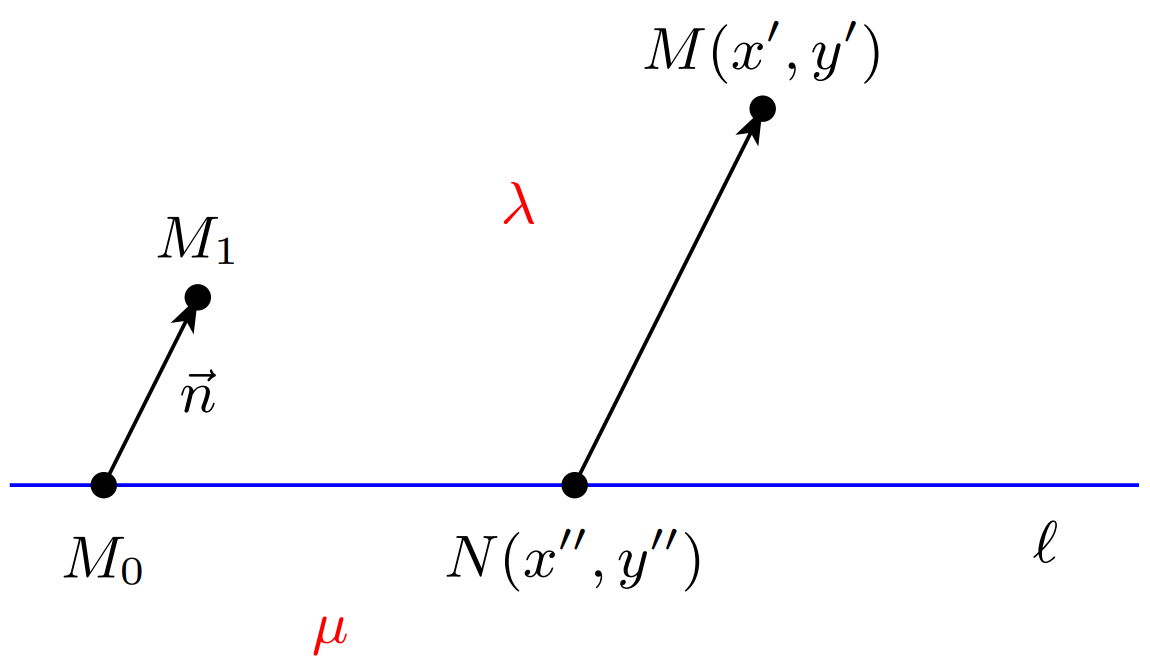
\includegraphics[width=11cm]{t7}

\textbf{Доказательство}. Пусть $M \in \lambda$. Через точку М проведём прямую, коллинеарнубю $\vec{n}$. Мы знаем, что \textit{главный вектор прямой не коллинеарен этой прямой}. Значит наша прямая пересечёт $l$. Пусть точка пересечения это $N(x'', y'')$. Очевидно $Ax'' + By'' + C = 0$. $\overrightarrow{NM}$ и $\vec{n}$ сонаправлены, то есть $\overrightarrow{NM} = t \vec{n}, t>0$. Получаем, что $x' -x'' = tA, y'-y'' = tB \Rightarrow x' = x'' + tA, y' = y'' + tB \Rightarrow$ \newline \begin{equation}
Ax' + By' + C = A(x'' + tA) + B(y'' + tB) + C = Ax'' + By'' + C + t(A^2 + B^2) = t(A^2+B^2)>0
\end{equation}
Мы доказали, что если $M \in \lambda$, то $Ax' + By' + C > 0$. 

Ребят, ну давайте второе утверждение докажете сами плз.
\newline
Точки $P(x_1, y_1)$ и $Q(x_2, y_2)$ лежат по одну сторону от прямой $Ax+By+C=0$ тогда и только тогда, когда $sgn (Ax_1+By_1+C) = sgn (Ax_2+By_2+C)$ и по разные стороны, когда $sgn (Ax_1+By_1+C) \neq sgn (Ax_2+By_2+C)$



\section*{Плоскость}

$\sigma$ - плоскость, $M_0(x_0, y_0, z_0)$ - точка в $\sigma$, $\vec{a_1} = (q_1, r_1, s_1)$ и $\vec{a_2} = (q_2, r_2, s_2)$ - направляющие вектора, не коллинеарные между собой.
$\overrightarrow{M_0M_1} = u\vec{a_1} + v\vec{a_2}$, где $u, v \in \mathbb{R}$.


Уравнения плоскости: \begin{enumerate}
\item Параметрическое; $
\begin{cases}
   x = x_0 + q_1u + q_2v 
   \\
   y = y_0 + r_1u + r_2v
   \\
   z = z_0 + s_1u + s_2v  
 \end{cases}
$
\item Каноническое: $\begin{vmatrix}
	x-x_0& y-y_0& z-z_0\\
	q_1& r_1& s_1\\
	q_2& r_2& s_2
\end{vmatrix} = 0$

\item Общее: из канонического можем получить $A = \begin{vmatrix}
	r_1& s_1\\
	r_2&s_2
\end{vmatrix}$, $B = \begin{vmatrix}
	q_1& s_1\\
	q_2&s_2
\end{vmatrix}$, $C = \begin{vmatrix}
	q_1& r_1\\
	q_2&r_2
\end{vmatrix}$. Имеем $A(x-x_0)+B(y-y_0)+C(z-z_0) = 0$ и $(A,B,C) -$  главный	 вектор плоскости.
\end{enumerate}

\textbf{Теорема}. Любая плоскость представима в виде уравнения $Ax+By+Cz+D=0$. И наоборот, любое уравнение $Ax+By+Cz+D=0$ задаёт плоскость.

\textbf{Доказательство}. \begin{enumerate}
\item Любая плоскость представима каноническим уравнением $\begin{vmatrix}
	x-x_0& y-y_0& z-z_0\\
	q_1& r_1& s_1\\
	q_2& r_2& s_2
\end{vmatrix} = 0$\newline

$\begin{vmatrix}
	r_1& s_1\\
	r_2&s_2
\end{vmatrix}(x-x_0)+ \begin{vmatrix}
	q_1& s_1\\
	q_2&s_2
\end{vmatrix} (y-y_0)+ \begin{vmatrix}
	q_1& r_1\\
	q_2&r_2
\end{vmatrix} (z-z_0) = 0$, где $A(x-x_0)+B(y-y_0)+C(z-z_0) = 0$ и $(A,B,C)$.

\item Возьмём уравнение $Ax+By+Cz+D=0, A^2 + B^2 + C^2 \neq 0$.
\begin{enumerate}
\item Возьмём точку $(x_0, y_0, z_0)$, удовлетворяющую данному уравнению.

Если $A\neq 0$, то берём $y_0 = z_0 = 0$ и получаем $\displaystyle x_0 = \frac{D}{A}$ (аналогично для $A=0$, тогда либо $B \neq 0$, либо $C \neq 0$.

\item Возьмём 2 вектора: 

\begin{itemize}
\item $\vec{a_1} = (-B, A, 0)$
\item $\vec{a_2} = (-C, 0, A)$
\end{itemize}

Составим каноническое уравнение плоскости, проходящей через $M_0$ с направляющими векторами $a_1$ и $a_2$.

$\begin{vmatrix}
	x-x_0& y-y_0& z-z_0\\
	-B& A& 0\\
	-C& 0& A
\end{vmatrix} = 0$

\begin{equation}
A^2(x-x_0) + AB(y-y_0)+AC(z-z_0) = 0|:A \Rightarrow A(x-x_0) + B(y-y_0)+C(z-z_0) = 0 
\end{equation}
\begin{equation}
Ax+By+Cz - Ax_0 - By_0 -Cz_0 = 0
\end{equation}
Здесь $D = - Ax_0 - By_0 -Cz_0$.

\end{enumerate}
\end{enumerate}

\section*{Взаимное расположение плоскостей}
Пусть плоскости заданы уравнениями \begin{enumerate}
\item $\pi_1: A_1x+B_1y+C_1z+D_1 = 0$
\item $\pi_2: A_2x+B_2y+C_2z+D_2 = 0$
\end{enumerate}

Тогда\begin{enumerate}
\item $\pi_1$ и $\pi_2$ пересекаются $\displaystyle \Leftrightarrow \frac{A_1}{A_2} \neq \frac{B_1}{B_2}$ или $\displaystyle \frac{A_1}{A_2} \neq \frac{C_1}{C_2}$

\item $\pi_1 \parallel \pi_2$ и $\pi_1 \neq \pi_2 \Leftrightarrow \displaystyle \frac{A_1}{A_2} = \frac{B_1}{B_2} = \frac{C_1}{C_2} \neq \frac{D_1}{D_2}$
\end{enumerate}

\textbf{Доказательство (в общем случае)}. Рассмотрим систему уравнений
\begin{equation}
\begin{cases}
   A_1x+B_1y+C_1z+D_1 = 0
   \\
   A_2x+B_2y+C_2z+D_2 = 0
 \end{cases}
\end{equation}
Пусть для определения $\displaystyle \frac{A_1}{A_2} \neq \frac{B_1}{B_2}$.

Давайте сделаем $z_0=0$, тогда получим систему \begin{equation}
\begin{cases}
   A_1x+B_1y = -D_1
   \\
   A_2x+B_2y= -D_2
 \end{cases} (*)
\end{equation}
Эта система по правилу Крамера имеет единственное решение $(x_0, y_0)$. Значит невозможно $\pi_1 = \pi_2$.

Если $\pi_1 = \pi_2$, то имеется другое решение системы, что противоречит с тем, что система $(*)$ имеет только одно решение.

$\begin{cases}
   A_1x+B_1y+C_1z+D_1 = 0
   \\
   A_2x+B_2y+C_2z+D_2 = 0
 \end{cases}$
 
$\displaystyle \frac{A_1}{A_2} = \frac{B_1}{B_2} = \frac{C_1}{C_2} = t$, откуда $\begin{cases}
   tA_2x+tB_2y+tC_2z+D_1 = 0
   \\
   tA_2x+tB_2y+tC_2z+tD_2 = 0
 \end{cases} \Rightarrow D_1 = tD_2 = 0 \Rightarrow \displaystyle t = \frac{D_1}{D_2}$. Если это не так, то решений $\infty$.
 
\section*{Нормальное уравнение плоскости}

?????????????????????????????????

\section*{Отклонение точки от плоскости}

\textbf{Теорема (о полупространствах)}. Пусть $M(x', y', z')$ - произольная точка пространства. Если $M \in \lambda$, то $Ax' + By' + Cz' + D > 0$, а если $M \in \mu$, то $Ax' + By' + Cz' + D < 0$.

Точки $P(x_1, y_1, z_1)$ и $Q(x_2, y_2, z_2)$ расположены по одну сторону от плоскости\newline $Ax' + By' + Cz' + D = 0$ тогда и только тогда, когда\newline $sgn(Ax_1 + By_1 +Cz_1+D = sgn(Ax_2 + By_2 + Cz_2 + D$, и по разные стороны, когда\newline $sgn(Ax_1 + By_1 +Cz_1+D \neq sgn(Ax_2 + By_2 + Cz_2 + D$.

\section*{Виды уравнений прямой в пространстве}

Пусть на прямой $l$ лежит точка $M_0(x_0,y_0,z_0)$, $\vec{a} = (q,r,s) \neq \vec{0}$ - направляющий вектор прямой $l$. $\vec{r_0}$ - радиус-вектор точки $M_0$.

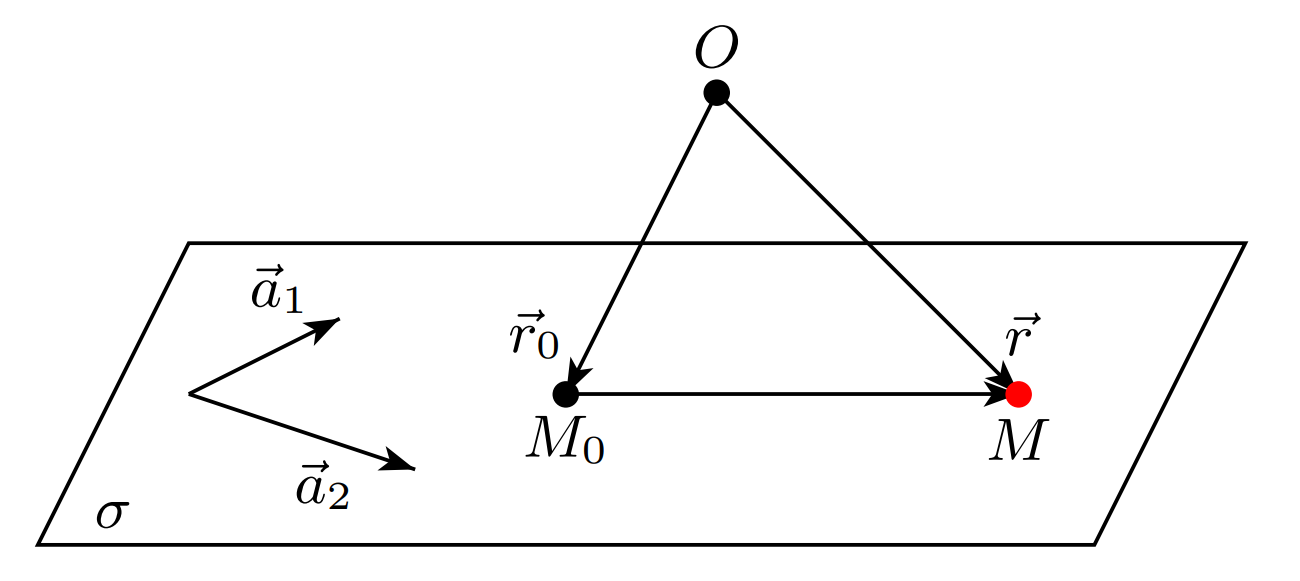
\includegraphics[width=10cm]{t8}

Точка $M$ лежит на $l$ тогда и только тогда, когда $\vec{a}$ коллинеарен $\overrightarrow{M_0M}$, то есть $\overrightarrow{M_0M}  = t\vec{a}$.

$M \in l \Leftrightarrow \vec{r} = \vec{r_0} + t\vec{a}$.

Виды уравнений прямой в пространстве:
\begin{enumerate}
\item Векторное: $\vec{r} = \vec{r_0} + t\vec{a}$
\item Параметрическое: $\begin{cases}
   x=x_0+qt
   \\
   y=y_0+rt
   \\
   z=z_0+st
 \end{cases}$
\item Каноническое: $\displaystyle \frac{x-x_0}{q} = \frac{y-y_0}{r} = \frac{z-z_0}{s}$
\item По двум точкам: $\displaystyle \frac{x-x_0}{x_1-x_0} = \frac{y-y_0}{y_1-y_0} = \frac{z-z_0}{z_1-z_0}$
\item Общие уравнения (как пересечение двух плоскостей): $\begin{cases}
A_1x+B_1y+C_1z+D_1=0,
\\
A_2x+B_2y+C_2z+D_2=0
\end{cases}$
\end{enumerate}

\textbf{Теорема}. Любая прямая в пространстве представима общим уравнением.

\textbf{Доказательство.} 

У нас плосоксти пересекаются, поэтому нормальные векторы плоскостей непараллельны.

Общий случай. Предположим $\displaystyle \frac{A_1}{A_2} \neq \frac{B_1}{B_2}$.
 
 Перепишем систему в виде $\begin{cases}
 A_1x+B_1y=-C_1z-D_1,
 \\
 A_2x+B_2y=-C_2z-D_2
 \end{cases}
$ Зафиксируем $z$ и скажем, что $z=t$: $\displaystyle \begin{cases}
 A_1x+B_1y=-C_1t-D_1,
 \\
 A_2x+B_2y=-C_2t-D_2
 \end{cases}
$

Поскольку $\displaystyle \begin{vmatrix}
A_1& A_2\\
B_1& B_2
\end{vmatrix} \neq 0$, то при любом $t$ система имеет единственное решение по правилу Крамера: \begin{equation}
\displaystyle
\begin{cases}
x=\frac{\begin{vmatrix}
-C_1t-D_1& A_2\\
-C_2t-D_2& B_2
\end{vmatrix}}{\begin{vmatrix}
A_1& A_2\\
B_1& B_2
\end{vmatrix}} = \frac{\displaystyle t(-B_2C_1+A_2C_2) - B_2D_1+A_2D_2}{\begin{vmatrix}
A_1& A_2\\
B_1& B_2
\end{vmatrix}} = \frac{\displaystyle -B_2D_1+A_2D_2}{\begin{vmatrix}
A_1& A_2\\
B_1& B_2
\end{vmatrix}} + t\frac{\displaystyle -B_2C_1+A_2C_2}{\begin{vmatrix}
A_1& A_2\\
B_1& B_2
\end{vmatrix}},
\\
y=\frac{\begin{vmatrix}
-A-1& C_1t-D_1\\
-B_1& C_2t-D_2
\end{vmatrix}}{\begin{vmatrix}
A_1& A_2\\
B_1& B_2
\end{vmatrix}} = \frac{\displaystyle t(-A_1C_2+B_1C_1) - A_1D_2+B_1D_1}{\begin{vmatrix}
A_1& A_2\\
B_1& B_2
\end{vmatrix}} = \frac{\displaystyle -A_1D_2+B_1D_1}{\begin{vmatrix}
A_1& A_2\\
B_1& B_2
\end{vmatrix}} + t\frac{\displaystyle -A_1C_2+B_1C_1}{\begin{vmatrix}
A_1& A_2\\
B_1& B_2
\end{vmatrix}},
\\ 
z = t
 \end{cases}
\end{equation}

\begin{equation}
\displaystyle
\begin{cases}
x=\frac{\displaystyle -B_2D_1+A_2D_2}{\begin{vmatrix}
A_1& A_2\\
B_1& B_2
\end{vmatrix}} + t\frac{\displaystyle -B_2C_1+A_2C_2}{\begin{vmatrix}
A_1& A_2\\
B_1& B_2
\end{vmatrix}},
\\
y=\frac{\displaystyle -A_1D_2+B_1D_1}{\begin{vmatrix}
A_1& A_2\\
B_1& B_2
\end{vmatrix}} + t\frac{\displaystyle -A_1C_2+B_1C_1}{\begin{vmatrix}
A_1& A_2\\
B_1& B_2
\end{vmatrix}}
\\ z = t
 \end{cases}
\end{equation}


В ПСК можно доказать обратное: любое уравнение задаёт некоторую прямую\newline $\begin{cases}
A_1x+B_1y+C_1z+D_1=0,
\\
A_2x+B_2y+C_2z+D_2=0
\end{cases}$.

Поскольку плоскости непараллельны, то пусть $\displaystyle \frac{A_1}{A_2} \neq \frac{B_1}{B_2}$. Тогда берём $z=0$ и получаем систему $\begin{cases}
A_1x+B_1y=-D_1,
\\
A_2x+B_2y=-D_2
\end{cases}$, которая по правилу Крамера имеет единственное решение $(x_0, y_0)$.\newline Таким образом, точка с координатами $M(x_0, y_0, z_0)$ лежит на данной прямой.

$\vec{a} = \vec{n_1} \times \vec{n_2}$

$\vec{a_1} \perp \vec{n_1}, \vec{a_2} \perp \vec{n_2}$

Таким образом, из уравнения плоскостей мы получаем напраляющий вектор данной прямой. По точке $M_0$ и направляющему вектору мы сможем восстановить прямую:
\begin{equation}
\displaystyle \frac{x-x_0}{B_1C_2-B_2C_1} = \frac{y-y_0}{A_1C_2-A_2C_1} = \frac{z}{A_2B_2-A_2B_1}
\end{equation}

\section*{Взаимное расположение прямых в пространстве}
Пусть даны $l_1$ и $l_2$, а $\vec{a_1} = (q_1, r_1, s_1)$ и $\vec{a_2} = (q_2, r_2, s_2)$ - направляющие векторы для этих прямых соответственно. Возьмём по одной точке $M_1(x_1, y_1, z_1)$ и $M_2(x_2, y_2, z_2)$ с каждой прямой.

Если прямые \textit{лежат в одной плоскости (либо совпадают, либо пересекаются)}, то смешанное произведение $\overrightarrow{M_1M_2}, \vec{a_1}, \vec{a_2}$ компланарны, то есть смешанное произведение равно нулю: $\displaystyle \begin{vmatrix}
x_2-x_2& y_2-y_2& z_2-z_1\\
q_1& r_1& s_1\\
q_2& r_2& s_2
\end{vmatrix} = 0$.

Прямые \textit{скрещиваются}$\displaystyle \Leftrightarrow \begin{vmatrix}
x_2-x_2& y_2-y_2& z_2-z_1\\
q_1& r_1& s_1\\
q_2& r_2& s_2
\end{vmatrix} \neq 0$.

Прямые \textit{параллельны или совпадают}: $\displaystyle \vec{a_1} \parallel \vec{a_2} \Leftrightarrow \frac{q_1}{q_2} = \frac{r_1}{r_2} = \frac{s_1}{s_2}$.


\section*{Взаимное расположение прямой и плоскости в пространстве}
\textbf{Теорема}. Предположим, что дана плоскость $Ax+By+Cz+D=0$, где $A^2+B^2+C^2+D^2\neq 0$, и прямая $\displaystyle l: \begin{cases}
x=x_0+qt,
\\
y=y_0+rt,
\\
z=z_0+st
\end{cases}$. \textbf{Тогда прямая и плоскость пересекаются $\mathbf{\Leftrightarrow Aq+Br+Cs \neq 0}$}

$A(x_0 + qt) + B(y_0 + rt) + C(z_0 + st) = 0 \Leftrightarrow \vec{n} \perp \vec{a}$

$Ax_0 + By_0 + Cz_0 + D + (Aq+Br+Cs)t=0$

Если $Aq+Br+Cs \neq 0$, то решение единственное: $\displaystyle t = \frac{-(Ax_0 + By_0 + Cz_0 + D)}{Aq+Br+Cs}$ и прямая с плоскостью имеют одну общую точку.

Итак: \begin{itemize}
\item $l$ лежит в плоскости $\Leftrightarrow \begin{cases}
Ax_0 + By_0 + Cz_0 + D = 0,
\\
Aq+Br+Cs=0,
\end{cases}$
\item $l$ параллельна плоскости $\Leftrightarrow \begin{cases}
Ax_0 + By_0 + Cz_0 + D \neq 0,
\\
Aq+Br+Cs=0,
\end{cases}$
\item $l$ пересекается с плоскостью $\Leftrightarrow Aq+Br+Cs\neq 0$
\end{itemize}



\section*{Построение поля комплексных чисел}
Пусть $a,b \in \mathbb{R}$.

Рассмотрим множесто пар вида $(a,b)$.

Введем операции сложения и умножения $z_1 + z_1 = (x_1+x_2,y_1+y_2), z_1 z_2 = (x_1 x_2 -y_2 y_2, x_1 y_2 + x_2 y_1)$

\textbf{Теорема}. Относительно введенных операций множество $\mathbb{C}$ является полем:
\begin{itemize}
\item 
	сложение:\begin{itemize}
	\item коммутативность
	\item ассоциативность
	\item $(0,0)$ - нейтральный
	\item $(-x,-y)$ - противоположный элемент
	\end{itemize}

\item 
	умножение: \begin{itemize}
	\item коммутативность
	\item ассоциативность
	\item $(1,0)$ - нейтральный
	\item обратный элемент существует, если $(x,y) \neq (0,0)$ или $\displaystyle x^2+y^2 \neq 0$: $z^{-1} = \left( \frac{x}{x^2+y^2},-\frac{y}{x^2+y^2} \right)$
		\end{itemize}
		
		
\end{itemize}


\section*{Алгебраическая форма комплексного числа}
$(x,y) = (x,0) + y(0,1) = x+iy$ - общепринятая запись комплексного числа.

$x+iy$ (x - вещественная часть, y - мнимая часть)

Для каждого $z = x+iy$ существует $\overline{z} = x-iy$ - сопряжённое.


\section*{Тригонометрическая форма комплексного числа}

Любая точка плоскости однозначно задается парой $(r, \phi)$, где $r$ - расстояние от точки до начала координат.

$\displaystyle \begin{cases}
x = r \cos \phi,
\\
y = r \sin \phi
\end{cases} \Rightarrow z = |z| (\cos \phi + i \sin \phi)$

$\phi$ называется аргументом числа $z$ ($\phi = argZ$)

\section*{Действия с числами в тригонометрической форме}

При умножении комплексных чисел модули умножаются, а углы складываются.

При делении модули делятся, а углы вычитаются.



\section*{Формула Муавра}
 $z^n = (r(\cos \phi + i \sin \phi))^n = r^n ( \cos(n \phi) + i \sin(n \phi)$

\section*{Извлечение корней из комплексных чисел
}
\textbf{Определение}. Корнем n-ой степени комплексного числа z называется число $w$ такое,\newline что $w^n = z$.


Пусть $z = r(\cos \phi + i \sin \phi)$

$w = \rho (\cos \psi + i \sin \psi)$

У нас должно быть $w^n = z$: $w^n = \rho^n (\cos (n \psi) + i \sin (n \psi))$

$\rho^n (\cos (n \psi) + i \sin (n \psi)) = r (\cos  \phi + i \sin \phi)$

Числа равны, а значит равны их модули $\rho^n = r \Rightarrow \rho = \sqrt[n]{r}$

$\cos (n \psi) + i \sin (n \psi) = \cos  \phi + i \sin \phi \Rightarrow \begin{cases}
\cos (n \psi) = \cos \phi,
\\
\sin (n \psi) = \sin \phi
\end{cases}$.

Если у углов одинаковы $\cos$ и $\sin$, то углы различаются на $2\pi k, k \in \mathbb{Z}$:
\begin{equation}
n \psi = \phi + 2\pi k \Rightarrow \psi = \frac{\phi + 2 \pi k}{n} = \frac{\phi}{n} + \frac{2 \pi k}{n}
\end{equation}

$\displaystyle \psi_0 = \frac{\phi}{n}$

$\displaystyle \psi_1 = \frac{\phi}{n} + \frac{2\pi}{n}$

$\displaystyle \psi_2 = \frac{\phi}{n} + \frac{4\pi}{n}$

...

$\displaystyle \psi_{n-1} = \frac{\phi}{n} + \frac{2\pi}{n}n = \frac{\phi}{n} + 2\pi$

Таким образом, получаем, что аргументов для $w$, дающих разные корни $n-1$ степени в точности $n$ штук при $k =0, 1, ..., n-1$

$\psi = \frac{\phi}{n} + \frac{2\pi k}{n}, k = 0, 1, ..., n-1$.


Пусть $z = r(\cos \phi + i \sin \phi)$

\begin{equation}
\displaystyle w = \sqrt[n]{z} = \sqrt[n]{r} \left( \cos \frac{\phi + 2\pi k}{n} + i \sin \frac{\phi + 2\pi k}{n} \right), k = 0,1,...,n-1
\end{equation}

\textbf{В поле комплексных чисел любое комплексное число $z \neq 0$ имеет в точности $n$ корней $n$-ой степени (предыдущая формула)}

\textit{Пример. $\mathit{1 = \cos 0 + i \sin 0}$}

$\displaystyle \sqrt[3]{1} = \cos \frac{0+2\pi k}{3} + i \sin \frac{0 + 2\pi k}{3} = \cos \frac{2 \pi k}{3} + i \sin \frac{2 \pi k}{3}, k = 0,1,2$

$\displaystyle w_0 = \cos \frac{2 \pi 0}{3} + i \sin \frac{2 \pi 0}{3} = 1$

$\displaystyle w_1 = \cos \frac{2 \pi}{3} + i \sin \frac{2 \pi}{3} = -\frac{1}{2} + i\frac{\sqrt{3}}{2}$

$\displaystyle w_2 = \cos \frac{4 \pi}{3} + i \sin \frac{4 \pi}{3} = -\frac{1}{2} - i\frac{\sqrt{3}}{2}$\\

\textit{Пример. Корни n-ой степени из 1}

В случае $\mathbb{R}$: $\sqrt[n]{1} = 1$

В случае $\mathbb{C}$ мы имеем n корней:

$1 = 1(\cos 0 + i sin 0$
\begin{equation}
\displaystyle \sqrt[n]{1} = \sqrt[n]{1} \left( \cos \frac{2\pi k}{n} + i \sin \frac{2 \pi k}{n} \right), k=0,1,...,n-1
\end{equation}


При $k=0$: $w_0 = 1$

При $k=1$: $\displaystyle w_1 = \cos \frac{2\pi}{n} + i \sin \frac{2\pi}{n}$

$\displaystyle w_k = \cos \frac{2\pi k}{n} + i \sin \frac{2 \pi k}{n} = \left( \cos \frac{2\pi}{n} + i \sin \frac{2 \pi}{n} \right)^k = w^k$



\section*{Линейное пространство}
\textbf{Определение}. Множество V называется \textbf{линейным пространстом} над полем $\mathbb{F}$, если для каждой пары элементов V определена операция сложения и для каждого элемента $x \in V$ определена операция умножения на число $t \in \mathbb{F}$. При этом элементы V называются векторами, а элементы $\mathbb{F}$ называются скалярами.

Аксиомы:
\begin{enumerate}
\item $x+(y+z) = (x+y)+z$
\item $x+y=y+x$
\item $\exists 0: \forall x \in V 0 + x = x + 0 = x$
\item $\forall x \exists -x: x + (-x) = -x + x = 0$
\item $t(x+y) = tx + ty$
\item $(t+s)x = tx + sx$
\item $t(sx) = (ts)x$
\item $1x = x$
\end{enumerate}


Свойства:
\begin{enumerate}
\item Нулевой вектор единственный.
\item Противоположный элемент единственный
\end{enumerate}

Примеры линейных пространств:
\begin{enumerate}
\item Множество векторов плоскости
\item Множество векторов пространства
\item Множество последовательностей длиный n из элементов $\mathbb{R}$
\item Многочлены от одной переменной, степени которых не превосходят n
\item Матрицы $n \cdot m$
\end{enumerate}

\section*{Линейная зависимость векторов}
\textbf{Лемма}. Если система векторов $x_1, x_2, ..., x_m$ содержит нулевой вектор, то она линейно зависима.

\textbf{Доказательство}. 

Пусть $\vec{x_k} = \vec{0}$
Тогда можно взять линейную комбинацию $0x_1 + 0x_2 + ... + 1x_k + ... + 0x_m = \vec{0} \Rightarrow$ система векторов линейно зависима чтд.

\textbf{Лемма}. Если к линейно зависимой системе добавить новые векторы, то система останется линейно зависимой.

\textbf{Доказательство}. 

Пусть  $x_1, x_2, ..., x_m$ - линейно зависимая система. Тогда некоторый $\vec{x_k}$ выражается через остальные $x_1, ..., x_{k-1}, x_{k+1}, ..., x_m$. Если мы добавим еще какие-то векторы в системы, то $\vec{x_k}$ всё равно будет выражаться через остальные вектора. Пусть мы добавили веткоры $y_1, y_2, y_l$. Тогда $\vec{x_k} = t_1x_1 + ... + t_mx_m + 0y_1 +0y_2 + ... + 9y_l$ чтд.


\textbf{Лемма}. Если система ненулевых векторов $a_1, ..., a_m$ линейно зависима, то найдется $a_k$ который выражается через предыдущие векторы.

\textbf{Доказательство}. По условию существуют скаляры $t_1, t_2, ..., t_k$, по крайней мере один из которых не равен 0, такие, что $t_1a_1 + t_2a_2 + ... + t_ka_k = 0$.

Пусть j - наибольший индекс, для которого $t_j \neq 0$. Если $j=1$, то равенство  $t_1a_1 + t_2a_2 + ... + t_ka_k = 0$ сводится к $t_1a_1 = 0$, откуда $a_1 = 0$, противоречие. Тогда $j>1$.

Перенося последнее слагаемое в другуб часть и деля на $t_j \neq 0$ получаем \begin{equation}
\displaystyle a_j = -\frac{t_1}{t_j}\cdot a_1 - ... - \frac{t_{j-1}}{a_j} \cdot a_{j-1}
\end{equation}
чтд браток.

\section*{Системы образующих}
\textbf{Определение}. Система векторов $\Sigma$ векторного пространства V называется \textbf{системой образующих} этого пространства, если любой вектор из V линейно вырадатеся через какие-то вектора из системы $\Sigma$.

\section*{Базис линейного пространства}
\textbf{Определение. Базисом} векторного пространства называется линейно независимая
система образующих.


\textbf{Замечание 1.} Система векторов $e_1, e_2, ..., e_n$ линейно независима.

\textbf{Доказательство.} Предположим, что $x_1e_1+x_2e_2 + ... + x_ne_n = 0$, для некоторых $x_1, ..., x_n \in \mathbb{F}$. 

$x_1e_1+x_2e_2 + ... + x_ne_n = (x_1, x_2, ..., x_n)$, то есть $(x_1, x_2, ..., x_n) = 0 \Leftrightarrow x_1 = x_2 = ... = x_n = 0$

\textbf{Замечание 2.} Если $x = (x_1, x_2, ..., x_m) $ - произвольный вектора из $F^n$, то $x = x_1e_1 + x_2e_2 + ... + x_ne_n$

\textbf{Замечание 3.} Вектора $e_1, e_2, ..., e_n$ образуют базис пространства $F^n$.

\textbf{Доказательство.} В силу 1 и 2 замечания эти вектора линейно независимы и являются системой образующих пространства $F^n$.

\textbf{Определение}. Система векторов $e_1, e_2, ..., e_n$ называется \textbf{стандартным базисом} пространства $F^n$.

\section*{Равномощность базисов}

\textbf{Теорема}. Если в векторном пространстве есть базис из n векторов, то и любой базис этого пространства содержит ровно n векторов.

\textbf{Доказательство.} Пусть $A := (a_1, a_2, ..., a_n) - $ базис пространства, а $B := (b_1, b_2, ..., b_k)$ - другой базис. Чтобы доказать, что $n=k$, в силу симметрии достаточно проверить, что $k \leq n$. Пусть $k > n$.

Рассмотрим систему $b_1, a_1, a_2, ..., a_n$.

Это линейно зависимая система ненулевых векторов, так как вектор $b_1$ выражается через систему образующих А. По лемме о правом крайнем в $b_1, a_1, a_2, ..., a_n$ есть вектор, который линейно выражается через предыдущие. Это не может быть векторв $b_1$ - у него нет предыдущих. Значит, это какой-то $a_i$. Выкинув его, получим систему $b_1, a_1, a_2, ..., a_{i-1}, a_{i+1}, ..., a_n $ (*), которая останется системой образующих согласно лемме о прополке.

Теперь рассмотрим $b_2, b_1, a_1, a_2, ..., a_n$ (**).

Это линейно незавимимая система ненулевых векторов, так как вектор $b_2$ выражается через систему образующих (*). По лемме о правом крайнем в (**) есть вектор, выражаюшийся через предыдущие. Это не может быть ни $b_1$, ни $b_2$ (у $b_2$ нет предыдущих, а $b_1$ не выражается через $b_2$, так как система B линейно независимая). Значит, это какой-то $a_j, j \neq i$.

Выкинув его из (**), получим систему $b_2, b_1, a_1, a_2, ..., a_{i-1}, a_{i+1}, ..., a_{j-1}, a_{j+1}, ...,a_n$, которая останется системой образующих согласно лемме о прополке. Продолжая добавлять вектора из B и удалять вектора из А, будем получать системы из n образующих, в которых всё больше вектораов из B и всё меньше из А. Поскольку $k>n$, то через n шагов мы придём к системе образующих $b_n, ..., b_2, b_1$. Но тогда вектор $b_{n+1}$ выражается через эту систему обазующих, что противоречит линейной незавимисости B. чтд браток.


\textbf{Следствия.}
\begin{itemize}
\item Если у векторного пространства V есть система из n образующих, то любая линейно независимая система в V содержит не больше n векторов.
\item  Если в V есть линейно независимая система из n векторов, то любая система образующих пространства V содержит не менее n векторов.
\end{itemize}





\section*{Размерность пространства}
Если у векторного пространства есть конечный базис, то число векторов в базисе называется \textbf{размерностью} этого пространства.
Размерность пространства V обозначается через $dim V$.

\textbf{Теорема о разложении вектора по базису}. Пусть V - ненулевое векторное пространство, $a_1, a_2, ..., a_n$ - базис. Тогда $\forall x \in V$ существуют единственные $t_1, t_2, ..., t_n$ такие, что $x = t_1a_1 + t_2a_2 + ... + t_na_n (*)$.

\textbf{Доказательство.} Сущестование $t_1, t_2, ..., t_n$ ясно, поскольку базис - система образующих. Предположим, что наравне с (*) выполняется $x = s_1a_1 + s_2a_2 + ... + s_na_n$ для некоторых скаляров $s_i$. Вычтем одно равенство из другого и получим: \begin{equation}
(t_1-s_1)a_1 + (t_2-s_2)a_2 + ... + (t_n-s_n)a_n = 0
\end{equation}

Поскольку вектора $a_i$ линейно независимы, получаем, $t_i-s_i = 0 \Rightarrow t_i = s_i$ чтд браток.



\section*{Координаты вектора}
\textbf{Определение}. Равенство $x = t_1a_1 + t_2a_2 + ... + t_na_n$ называется \textbf{разложением вектора }
x \textbf{по базису} $a_1, a_2, ..., a_n$. Скаляры $t_1, t_2, ..., t_n$ называются координатами вектора x в базисе $a_1, a_2, ..., a_n$. Записывается $x = (t_1, t_2, ..., t_n)$. 

\section*{Действия с векторами в координатной форме}



\section*{Подпространства линейного пространства}
\textbf{Определение.} Непустое подмножество M векторного пространства V над полем F
называется \textbf{подпространством} пространства V , если выполняются
следующие условия:
\begin{enumerate}
\item если $x,y \in M$, то $x+y \in M$ (замкнутость подпространства относительно сложения векторов).
\item если $x \in M, t \in F$ то $tx \in M$ (замкнутость подпространства относительно умножения вектора на скаляр).
\end{enumerate}


\textbf{Определение}. Векторные пространства $V_1$ и $V_2$ над одним и тем же полем $F$ изоморфны, если существует биекция $f$ из $V_1$ на $V_2$ (называемая изоморфизмом) такая, что $f$ сохраняет операции, т.е. 

\begin{equation}
\forall x_1, x_2 \in V_1 \forall t \in F \quad f(x_1+x_2) = f(x_1) + f(x_2) \quad \& \quad f(tx) = t \cdot f(x)
\end{equation}

\textbf{Теорема об изоморфизме векторных пространств}. Любое n-мерное векторное пространство V над полем F изоморфно
пространству $F^n$.

\textbf{Доказательство.} Пусть $a_1, a_2, ..., a_n$ - базис пространства $V, b \in V, (t_1, ..., t_n) - $ координаты вектора $b$ в этом базисе. Определим отображение $f: V \rightarrow F^n$ правилом: $f(b) := t_1, ..., t_n)$. Поскольку координаты определяют вектор однозначно, то отображение $f$ инъективно. Сюръективность $f$ очевидна: если $y = (s_1, ..., s_n) \in F^n$, то $y = f(x)$, где $x = s_1a_1 + s_2a_2 + ... + s_na_n$.

Наконец, сохранение операций вытекает из замечания о координатах суммы векторов и произвежения вектора на скаляр. 

Таким образом, $f$ - изоморфизм из $V$ на $F^n$. чтд браток.

\section*{Операции над подпространствами и их свойства}

Нулевой вектор содержится в любом подпространстве M пространства V.
\textbf{Доказательство.} Если $x$ - произвольный вектор из М, то по второму условию из определения подпространства $0 = 0 \cdot x \in M$.

\textbf{Замечание о подпространстве, порождённом набором векторов}. Пусть V - векторное пространство и $a_1, a_2, ..., a_k \in V$. Тогда $<a_1, ..., a_k>$ - наименьшее подпространство пространства V, содержащее вектора $a_1, ..., a_k$.

\textbf{Доказательство}. Пусть M – подпространство пространства V , содержащее
вектора $a_1, a_2, ..., a_k$. По определению подпространства любая линейная
комбинация векторов$a_1, a_2, ..., a_k$ лежит в M. Следовательно,
$<a_1, ..., a_k> \subseteq M$. чтд браток.

\textbf{Предложение о размерности подпространства}. 
Пусть M – подпространство векторного пространства V . Тогда
$dim M \leq dim V$ , причем $dim M = dim V$ тогда и только тогда, когда
M = V.

\textbf{Доказательство}. Если M или V – нулевое пространство, то оба
утверждения предложения выполняются тривиальным образом. Будем
поэтому считать, что M и V – ненулевые пространства. Пусть $dim M = k$,
$dim V = n$. Неравенство $k \leq n$ следует из того, что базис M – это линейно
независимая система в V , а любую линейно независимую систему
векторов из V можно дополнить до базиса V по теореме о продолжении. При этои для дополнения нужно $n-k$ векторов. Поэтому если $n=k$, то базис M уже является базисом V , т.е. $M = V$ . Обратное утверждение очевидно.

\textbf{Определение}. Пусть V – векторное пространство, а $M_1$ и $M_2$ – его подпространства.
Сумма подпространств $M_1$ и $M_2$ – это множество $M_1$ + $M_2$ всех сумм
векторов из $M_1$ с векторами из $M_2$:
\begin{equation}
M_1+M_2 := \{ x_1 + x_2: x_1 \in M_1, x_2 \in M_2 \}
\end{equation}

\textbf{Замечание о сумме и пересечении подпространств}. Если $M_1$ и $M_2$ - подпространства V, то $M_1+M_2$ и $M_1 \bigcap M_2$ также являются подпространствами V.

\textbf{Доказательство.} В силу замечания о нулевом векторе и подпространствах,
каждое из подпространств $M_1$ и $M_2$ содержит нулевой вектор. Следовательно, $0=0+0 \in M_1+M_2$ и $0 \in M_1 \cap M_2$. В частности, множества $M_1+M_2$ и $M_1 \cap M_2$ непустые.

Пусть $x, y \in M_1+M_2$ и $t$ - скаляр. Тогда $x=x_1+x_2, y=y_1+y_2$ для некоторых $x_1, y_1 \in M_1$ и $x_2, y_2 \in M_2$. Получаем \begin{equation}
x+y = (x_1+x_2) + (y_1+y_2) = (x_1+y_1)+(x_2+y_2) \in M_1 + M_2, tx = t(x_1 + x_2) = tx_1 + tx_2 \in M_1 + M_2
\end{equation}

Итак, $M_1+M_2$ -подпространство в V. Далее пусть $x, y \in M_1 \cap M_2$ и $t$ - скаляр. Тогда $x, y \in M_1$ и $x, y \in M_2$. При этом имеем $x+y \in M_1, x+y \in M_2, tx \in M_1, tx \in M_2 \Rightarrow x+y \in M_1, x+y \in M_2, tx \in M_1 \cap M_2$, то есть $M_1 \cap M_2$ - подпространство V. чтд браток.

\textbf{Замечание о сумме подпространств}. Если $M_1$ и $M_2$ – подпространства пространства V , то $M_1 + M_2$ –
наименьшее подпространство в V , содержащее $M_1$ и $M_2$.

\textbf{Доказательство}. Если $x \in M_1$, то $x \in M_1 + M_2$, поскольку $x = x + 0, 0 \in M_2$. Следовательно, $M_1 \subseteq M_1 + M_2$. Аналогично, $M_2 \subseteq M_1 + M_2$. Тогда $x = x_1 + x_2$ для некоторых $x_1 \in M_1$ и $x_2 \in M_2$. Следовательно, $x_1, x_2 \in M$, откуда $x=x_1+x_2 \in M$. Итак $M_1 + M_2 \subseteq M$. чтд браток.

\textbf{Теорема о размерности суммы и пересечения подпространств}. Пусть V – векторное пространство, а $M_1$ и $M_2$ – его подпространства.
Тогда размерность суммы подпространств $M_1$ и $M_2$ равна сумме размерностей этих подпространств минус размерность их пересечения. 

\textbf{Доказательство.} Из предложения о размерности подпространства $dim(M_1 \cap M_2) \leq dim M_1$ и $dim(M_1 \cap M_2) \leq dim M_2$.

Положим $dim(M_1 \cap M_2) = k, dim M_1 = k + l, dim M_2 = k + m$. Если $M_1 = \{ 0 \}$, то очевидно $dim(M_1 \cap M_2) = \{ 0 \}, M_1 + M_2  = M_2$ и потому 
\begin{equation}
dim(M_1 + M_2) = dim M_2 = dim M_1 + dim M_2 - dim(M_1 \cap M_2)
\end{equation}
Аналогично разбирается случай $M_2 = \{ 0 \} $. 

Далее можно считать, что $M_1$ и $M_2$ ненулевые и $M_1 \cap M_2 \neq \{ 0 \}$. Пусть $a_1, .. a_k$ - базис $dim(M_1 \cap M_2)$.

По теореме о продолжении $a_1, .. a_k$ можно дополнить как до базиса $M_1$, так и до $M_2$. Пусть $a_1, .. a_k, b_1, .., b_l$ - базис $M_1$, а $a_1, .. a_k,c_1, c_2, ..., c_m$ - базис $M_2$.

Докажем, что базис $a_1, .. a_k, b_1, ..., b_l, c_1, ..., c_m$ является базисом пространства $M_1 + M_2$. Этого достаточно для доказательства теоремы, так как число векторов в этом наборе равно \begin{equation}
k + l + m = (k+l) + (k+m) - k = dim M_1 + dim M_2 -dim (M_1 \cap M_2)
\end{equation}

Пусть $x \in M_1 + M_2$. Тогда $x = x_1 + x_2$. $x_1 $- лин. комбинация векторов $a_1, .. a_k, b_1, .., b_l$, а $x_2$ - лин комбинация векторов $a_1, .. a_k,c_1, c_2, ..., c_m$.

Отсюда $x$ - лин. комбинация $a_1, .. a_k, b_1, ..., b_l, c_1, ..., c_m$. 

Таким образом, $a_1, .. a_k, b_1, ..., b_l, c_1, ..., c_m$ - система образующих пространства $M_1 + M_2$. Осталось доказать, что эта система линейно независима.

Предположим, что
 \begin{equation}
t_1a_1 + t_2a_2 + ... +t_ka_k + s_1b_1 + ... + s_lb_l + ... + r_1c_1 + r_2c_2 + ... + r_mc_m = 0
\end{equation} 
Нужно доказать, что все эти скаляры равны нулю.

Положим $y = s_1b_2 +s_2b_2 + ... + s_lb_l$. Очев $y \in M_1$. С другой стороны из (28) вытекает, что \begin{equation}
y = -t_1a_1 - t_2a_2 -... -t_ka_k - r_1c_1 -r_2c_2 -.. -r_mc_m \in M_2
\end{equation}

Следовательно $y \in M_1 \cap M_2$. Тогда $y$ - это линейная комбинация $a_1, ..., a_k$. То есь существуют такие скаляры $q_1, q_2, ..., q_k$, что 
\begin{equation}
y = s_1b_1+s_2b_2+...+s_lb_l = q_1a_1 + q_2a_2 + ... + q_ka_k
\end{equation}
Следовательно 
\begin{equation}
q_1a_1 + q_2a_2 + ... + q_ka_k - s_1b_1 - s_2b_2-... - s_lb_l = 0
\end{equation}

Покскольку $a_1, a_2, ..., a_k, b_1, ..., b_l$ образуют базис пространства $M_1$, то они линейно независимы. Поэтому линейная комбинация (31) тривиальна. Следовательно, равенство (28) принимает вид $t_1a_1 +t_2a_2 + ... + t_ka_k +r_1c_1 + r_2c_2 + ... + r_mc_m = 0$.

Учитывая, что вектора $a_1, .., a_k, c_1, ..., c_m$ образуют базис пространства $M_2$, получаем, что $t_1 = t_2 = ... = t_k = r_1 = ... = r_m = 0$. чтд браток.

\textbf{Опредление}. Пусть V – векторное пространство, а $M_1$ и $M_2$ – его подпространства.
Говорят, что сумма подпространств $M_1$ и $M_2$ является их \textbf{прямой суммой},
если $M_1 \cap M_2 =\{ 0 \}$. Прямая сумма подпространств $M_1$ и $M_2$
обозначается через $M_1 \oplus M_2$. 

\textbf{Замечание о базисе прямой суммы подпространств}. Если $V = M_1 \oplus M_2, b_1, b_2, ..., b_l - $базис $M_1$, а $c_1, c_2, ..., c_m$ - базис $M_2$, то $b_1, ..., b_l, c_1, ..., c_m$ - базис пространства V.

\textbf{Теорема о прямой сумме подпространств}. Пусть V – векторное пространство, а $M_1$ и $M_2$ – его подпространства. Следующие условия эквивалентны \begin{enumerate}
\item $M_1 + M_2$ является прямой суммой подпространств $M_1$ и $M_2$.
\item $dim(M_1+M_2) = dim M_1 + dim M_2$
\item любой вектор из $M_1+M_2$ единственным образом представим в виде суммы вектора из $M_1$ и вектора из $M_2$.
\item нулевой вектор пространства V единственным образом представим в виде суммы вектора из $M_1$ и вектора из $M_2$.
\end{enumerate}

\textbf{Доказательство.} Эквивалентность условий $1)$ и $2)$ непосредственно
вытекает из теоремы о размерности суммы и пересечения и того факта,
что размерность нулевого пространства равна 0. Импликация $3) \Rightarrow 4)$
очевидна. Поэтому достаточно доказать импликации $1) \Rightarrow 3)$ и $4) \Rightarrow 1)$.

\begin{itemize}
\item $1) \Rightarrow 3)$. Пусть $x \in M_1 + M_2$. По определению суммы подпространств $x = x_1 + x_2, x_1 \in M_1, x_2 \in M_2$. Остаётся доказать, то такое представление вектора x единственно. Предположим, что $x = y_1 + y_2, y_1 \in M_1, y_2 \in M_2$. Тогда мы имеем $x_1-y_1 = y_2 - x_2$. Ясно, что $x_1 - y_1 \in M_1, y_2-x_2 \in M_2$. Следовательно $x_1y_1 = y_2 - x_2 \in M_1 \cap M_2$.
Но $M_1 \cap M_2 = \{ 0 \}$. Поэтому $x_1y_1 = y_2 - x_2 = 0$, откуда $x_1 = y_1, x_2 = y_2$. чтд браток.

\item $4) \Rightarrow 1)$. Предположим, что $M_1 \cap M_2 \neq \{ 0 \}$, то есть существует ненулевой вектор $x \in M_1 \cap M_2$. Тогда вектор 0 может быть двумя различными способами представлен в виде суммы вектора из $M_1$ и вектора из $M_2$: $0 = x+(-x)$ и $0 = 0+0$. Мы получили противоречие с условием 4). чтд браток.
\end{itemize}

\textbf{Замечание о прямой сумме подпространств} \begin{equation}
V = M_1 \oplus M_2 \Leftrightarrow dim(M_1 + M_2) = dim M_1 + dim M_2 = dim V
\end{equation}
Необходимость сразу следует из теоремы о прямой сумме подпространств.
Достаточность следует из теоремы о размерности сумм и пересечения. чтд браток.

\textbf{Определение.}  Пусть $V = M_1 \oplus M_2$, $x \in V$. В силу теоремы о прямой сумме подпространств существуют однозначно определенные векторы $x_1 \in M_1$ и
$x_2 \in M_2$ такие, что $x = x_1 + x_2$. Вектор $x_1$ называется проекцией x на $M_1$
параллельно $M_2$, а вектор $x_2$ – проекцией x на $M_2$ параллельно $M_1$.
 


\textbf{Алгоритм нахождения проекции вектора на подпространство.} Пусть $V = M_1 \oplus M_2$, $x \in V$. Предположим, что нам известен базис $a_1, ..., a_k$ подпространства $M_1$ и базис $b_1, ..., b_l$ подпространства $M_2$. В силу замечания о базисе прямой суммы подпространств $a_1, a_2, ..., a_k, b_1, b_2, ... ,b_l$ - базис пространства $V$. Найдем координаты вектора x в этом базисе. Пусть они имеют вид $(t_1, ..., t_k, s_1, ..., s_l)$. Тогда $t_1a_1 + ... + t_ka_k + s_1b_1 + ... + s_lb_l$ - проекция x на $M_1$ параллельно $M_2$, а $s_1b_1 + ... + s_lb_l$ - проекция x на $M_2$ параллельно $M_1$.


\textbf{Определение.} Пусть V – векторное пространство, $x_0 \in V$ , а M – подпространство в V.
Множество всех векторов вида $x_0 + y$, где $y \in M$, называется \textbf{линейным
многообразием} в V и обозначается через $x_0 + M$. Вектор $x_0$ называется
\textbf{начальным вектором }многообразия $x_0 + M$, а подпространство M –
\textbf{направляющим подпространством} этого многообразия. Размерность
подпространства M называется размерностью многообразия $x_0 + M$.

Примеры
\begin{itemize}
\item Если $x_0 = 0$, то $x_0 + M = M$. Таким образом, всякое
подпространство пространства V является линейным многообразием в V
\item Если $M = \{ 0 \}$, то $x_0 + M = \{ x_0 \}$. Таким образом, всякий
вектор из V является линейным многообразием в V (размерности 0).
\item Обычные прямые и плоскости трехмерного пространства –
линейные многообразия.
\end{itemize}

\section*{Понятие линейного отображения}

Пусть V и W – векторные пространства над одним и тем же полем F.
Отображение $A: V \rightarrow W$ называется \textbf{линейным оператором}, если
для любых векторов $x1, x2 \in V$ и любого скаляра $t \in F$ выполняются
равенства $A(x_1+x_2) = A(x_1) + A(x_2), A(tx_1) = tA(x_1)$

Относительно первого равенства говорят, что A сохраняет сумму векторов,
относительно второго – что A сохраняет произведение вектора на скаляр.
Линейные операторы иначе называют линейными отображениями.

Важный специальный случай возникает, когда пространства V и W
совпадают, т.е. W = V . Тогда говорят, что A – линейный оператор
на пространстве V или что A – линейный оператор пространства V .
Линейные операторы на V иначе называют линейными преобразованиями.

\textbf{Свойства линейного оператора}
Пусть V и W – векторные пространства над полем F, а $A: V \rightarrow W$ –
линейный оператор. Тогда:
\begin{enumerate}
\item $A(0) = 0$
\item $A(\lambda_1v_1 + \lambda_2v_2 + ... + \lambda_mv_m) = \lambda_1A(v_1)+...+\lambda_m A(v_m)$ для любых векторов $v_1,v_2, ..., v_m \in V$ и любых скаляров $\lambda_1, ..., \lambda_m \in \mathbb{F}$.
\end{enumerate}

\textbf{Доказательство.} Первое свойство вытекает из того, что $A(0) = A(0 \cdot 0) = 0 \cdot A(0) = 0$.

Второе свойство выводится из определения линейного оператора очевидной индукцией по m. чтд браток доказательство огонь.

\textbf{Теорема существования и единственности линейного оператора}

Пусть V и W – векторные пространства над полем F, причем $dim V = n > 0$. Пусть $P = \{ p_1, ..., p_n \}$ - базис пространства $V$, а $w_1, ..., w_n$ - произвольные вектора из $W$.  Тогда существует
единственный линейный оператор $A: V \rightarrow W$ такой, что $A(p_i) = w_i$ для всех $i = 1, 2, ..., n$.

\textbf{Доказательство. Существование.} Пусть $x \in V$, а $(x_1, ..., x_n) - $ координаты вектора $x$ в базисе $P$. Определим оператор $A: V \rightarrow W$ правилом $A(x) := x_1w_1+x_2w_2+...x_nw_n$. В силу единственности координат вектора в базисе это определение корректно (т. е. образ вектора x под действием A определен однозначно). Из свойств координат суммы векторов и произведения вектора на скаляр вытекает, что этот оператор
линеен. Осталось заметить, что для всякого $i = 1,...n$ вектор $p_i$ имеет в базисе P координаты $(0,....,0,1,0,...,0)$, где единичка стоит на $i-$ом месте, и потому $A(p_i) = w_i$.

\textbf{Единственность.} Пусть $B: V \rightarrow W$ - линейный оператор такой, что $B(p_i) = w_i$ для всех $i = 1,...,n$. Пусть $x \in V$, а $(x_1, ..., x_n) - $ координаты вектора $x$ в базисе $P$. Тогда $x = x_1p_1 + ... + x_np_n$. В силу замечания о свойствах линейного оператора имеем
\begin{equation}
B(x) = B(x_1p_1 + ... + x_np_n) = x_1B(p_1) + ... + x_nB(p_n) = x_1w_1 + ... + x_nw_n = A(x)
\end{equation}

Следовательно $B=A$. чтд детка.





\section*{Произведение отображений}
\textbf{Определение} Пусть V и W – векторные пространства над полем F, $A: V \rightarrow W$ –
линейный оператор, а $t \in \mathbb{F}$. Произведением оператора A на скаляр t
называется оператор $B: V \rightarrow W$ задаваемый правилом $B(x) := tA(x)$ для
всех $x \in V$ . Произведение оператора A на скаляр t обозначается через $tA$.


\section*{Линейное пространство линейных отображений}
\textbf{Предложение о пространстве линейных операторов}.

Произведение линейного оператора на скаляр является линейным
оператором. Множество $Hom(V, W)$ с операциями сложения операторов
и умножения оператора на скаляр является векторным пространством.

\textbf{Доказательство}. Пусть $A,B \in Hom(V), x,y \in V, t, s \in \mathbb{F}$. Тогда
\begin{equation}
(tA)(x+y) = t(A(x+y)) = t(A(x) + A(y)) = tA(x) + tA(y) = (tA)(x) + (tA)(y)
\end{equation}

\begin{equation}
(tA)(sx) = t(A(sx)) = t(sA(x)) = (ts)(A(x)) = s(tA(x)) = s((tA)(x))
\end{equation}

Следовательно, $tA$ - линейный оператор.

Похожим образом получаем, что $1 \cdot A = A$. · A = A. С учетом свойств суммы операторов, мы получаем,
что в $Hom(V, W)$ выполнены все аксиомы векторного пространства. уничтожено.

\textbf{Теорема о пространствах линейных операторов и матриц}.

Если V и W – векторные пространства над полем F, $dim V = n$ и
$dim W = k$, то векторные пространства $Hom(V,W)$ и $F^{k\times n}$ изоморфны.

\textbf{Доказательство}. Зафиксируем в V базис $P = \{ p_1, p_2, . . . , p_n \}$, а в W –
базис $Q = \{ q_1, q_2, . . . , q_k \}$. Определим отображение
$\phi: Hom(V, W) \rightarrow F^{k \times n}$
правилом: если $A: V \rightarrow W$ – линейный оператор,
то $\phi(A)$ – матрица оператора A в базисах P и Q. Пусть $A, B \in Hom(V)$ и
$t \in F$. Надо проверить, что отображение $\phi$ биективно и выполнены равенства \begin{equation}
\phi (A+B) = \phi(A) + \phi(B)
\end{equation}
\begin{equation}
\phi(tA) = t \phi(A)
\end{equation}

В матрице $\phi(A+B)$ по столбцам записаны координаты векторов
$(A + B)(p_i)$ в базисе Q, а в матрицах $\phi(A)$ и $\phi(B)$ – координаты векторов
$A(p_i)$ и $B(p_i)$ соответственно в том же базисе. Поскольку
$(A + B)(p_i) = A(p_i) + B(p_i)$, координаты вектора $(A + B)(p_i)$ равны
сумме координат векторов $A(p_i)$ и $B(p_i)$. Первое из равенств \begin{equation}
\phi (A+B) = \phi(A) + \phi(B)
\end{equation}
\begin{equation}
\phi(tA) = t \phi(A)
\end{equation}
доказано. Второе из них проверяется вполне аналогично.

Проверим, что отображение $\phi$ биективно. Если $A, B \in Hom(V, W)$ и
$\phi(A) = \phi(B)$, то из определения матрицы линейного оператора вытекает,
что операторы A и B одинаково действуют на базисных векторах
пространства V . Но тогда $A = B$, так как линейный оператор однозначно
определяется своим действием на базисных векторах. Следовательно,
отображение $\phi$ инъективно.

Осталось доказать, что $\phi$ сюръективно. Пусть $A = (a_{ij}$) – произвольная
матрица размера $k \times n$. Для всякого $j = 1, 2, . . . , n$ положим
$w_j = a_{1j}q_1 + a_{2j}q_2 + · · · + a_{kj}q_k$. В силу теоремы существования и
единственности линейного оператора существует линейный оператор A
такой, что $A(p_i) = w_i$ для всех $i = 1, 2, . . . , n$. Из определения матрицы
оператора вытекает, что $A_{P,Q} = A$, т.е. $\phi(A) = A$. Следовательно, отображение $\phi$ сюръективно. убито фух.

\textbf{Следствие о размерности пространства линейных операторов}

Если V и W – векторные пространства над полем F, $dim V = n$ и
$dim W = k$, то $dim Hom(V, W) = kn$.

\section*{Свойства произведения}
\section*{Матрица линейного отображения}

\textbf{Определение}. Пусть $V$ и $W$ - векторные  пространства над полем F,\newline причем $dim V = n>0, dim W = k > 0$. Пусть $P = \{ p_1, ..., p_n \}$ - базис пространства $V$, а $Q = \{ q_1, ..., q_k \}$ - базис пространства $W$. \textbf{Матрицей линейного оператора } $A: V \rightarrow W$ \textbf{в базисах} $P$ и $Q$ называется $k \times n$ - матрица, итый столбец  которой состоит из координат вектора $A(p_i)$ в базисе $Q, i = 1, 2, ..., n$. Эта матрица обозначается $A_{P,Q}$ или просто $A$, если базисы зафиксированы.

Итак если \begin{equation}
\begin{matrix}
A(p_1) = a_{11}q_1 + a_{21}q_2 + ... + a_{k1}q_k,\\
A(p_2) = a_{12}q_1 + a_{22}q_2 + ... + a_{k2}q_k,\\
...\\
A(p_n) = a_{1n}q_1 + a_{2n}q_2 + ... + a_{kn}q_k,
\end{matrix}
\end{equation}
то $\displaystyle A_{P,Q} = \begin{pmatrix}
	a_{11}& a_{12}& ...& a_{1n}\\
	a_{21}& a_{22}& ...& a_{2n}\\
	...& ...& ...& ...\\
	a_{k1}& a_{k2}& ...& a_{kn}\\
\end{pmatrix}$
 
Если W = V, Q = P, то говорят о \textbf{матрице оператора в базисе} P.

\textbf{Определение.} Пусть V и W – векторные пространства над полем F, а A и B – линейные операторы из V в W. Суммой операторов A и B называется оператор $S : V \rightarrow W$, задаваемый правилом $S(x) := A(x) + B(x)$ для всех $x \in V$ .
Сумма операторов A и B обозначается через $A + B$.

Множество всех линейных операторов из V в W обозначается $Hom(V, W)$.

\textbf{Предложение о свойствах суммы операторов}. 

Сумма линейных операторов является линейным оператором. Множество
$Hom(V, W)$ с операцией сложения операторов является абелевой группой.

\textbf{Доказательство.} Пусть $A, B \in Hom(V), S = A+B$. $\forall x, y \in V, t \in \mathbb{F}$ имеем  \begin{equation}
S(x+y) = A(x + y) + B(x + y) = A(x) + A(y) + B(x) + B(y) = (A(x) + B(x)) +(A(y) + B(y))
= S(x) + S(y)
\end{equation}

\begin{equation}
S(tx) = A(tx) + B(tx) = tA(x) + tB(x) = t(A(x) + B(x))= tS(x)
\end{equation}

Следовательно, оператор S линеен.

Далее, если $A, B, C \in Hom(V,W)$, то \begin{equation}
(A+B)(x) = A(x) + B(x) = B(x) + A(x) = (B+A)(x)
\end{equation}
\begin{equation}
\begin{matrix}
((A+B)+C)(x) = (A+B)(x) + C(x) = (A(x) + B(x)) + C(x)=\\
 = A(x) + (B(x) + C(x)) = A(x) + (B+C)(x) = (A+(B+C))(x)
\end{matrix}
\end{equation}
 
Получается $A+B = B+A, (A+B)+C = A+(B+C)$. Нейтральным элементом по сложению является нулевой оператор O, поскольку $(A+O)(x) = A(x) + O(x) = A(x) + 0 = A(x)$

Обратным по сложению является оператор -A.

Предложение доказано. туда его.


\section*{}
\section*{}
\section*{}
\section*{}
\section*{}
\section*{}
\section*{}
\section*{}
\section*{}
\section*{}
\section*{}
\section*{}
\section*{}
\section*{}
\section*{}
\section*{}
\section*{}
\section*{}
\section*{}
\section*{}
\section*{}
\section*{}
\section*{}
\section*{}
\section*{}
\section*{}
\section*{}
\section*{}
\section*{}
\section*{}
\section*{}
\section*{}
\section*{}
\section*{}
\end{small}
}
\end{document}




